\documentclass[12pt]{article}

% TEMPLATE DEFAULT PACKAGES
\usepackage{amssymb,amsmath,amsfonts,eurosym,geometry,ulem,graphicx,color,setspace,sectsty,comment,natbib,pdflscape,array,adjustbox}

% ADDED PACKAGES FOR THIS MANUSCRIPT
\usepackage{palatino,newtxmath,multirow,titlesec,threeparttable,tabu,booktabs,titlesec,threeparttable,mathtools,bm,bbm,subcaption,pdflscape,tcolorbox,mathrsfs,tikz,float,longtable}
% endfloat,
% \usepackage[capposition=top]{floatrow}
\usepackage{tikzpagenodes}
\usepackage{pbox}

\usepackage{afterpage}
\usepackage[hyphens]{url}
\usepackage[margin=1cm]{caption}

\usepackage[draft]{hyperref}
\newcommand{\tim}{$\,\times\,$}
% FIGURES & TABLES CAPTION STYLING
\captionsetup[figure]{labelfont={bf},name={Figure},labelsep=period}
\captionsetup[table]{labelfont={bf},name={Table},labelsep=period}

% SECTION TITLE SETTINGS
\titlelabel{\thetitle.\enskip}
\titleformat*{\section}{\large\bfseries}
\titleformat*{\subsection}{\normalsize\bfseries}

% COLUMN TYPES
\newcolumntype{L}[1]{>{\raggedright\let\newline\\\arraybackslash\hspace{0pt}}m{#1}}
\newcolumntype{C}{>{\centering\arraybackslash}p{5.2em}}
\newcolumntype{D}{>{\centering\arraybackslash}p{5em}}
\newcolumntype{G}{>{\centering\arraybackslash}p{6em}}
\newcolumntype{R}[1]{>{\raggedleft\let\newline\\\arraybackslash\hspace{0pt}}m{#1}}


% MARGINS AND SPACING
\normalem
\geometry{left=1.1in,right=1.1in,top=1.0in,bottom=1.0in}
\setlength{\parskip}{2.5pt}

% SPECIAL CELL 
\newcommand{\specialcell}[2][c]{%
	\begin{tabular}[#1]{@{}l@{}}#2\end{tabular}}

% NO INDENT ON FOOTNOTES
\usepackage[hang,flushmargin]{footmisc}




\newcommand{\regtext}{
	``hm'' refers to a hectometer or 100 meters. Observations are one hectare plots ($\text{hm}^{2}$).
``Plot footprint'' is the effect of an additional hectare of overlap with constructed projects.  
For plots outside of projects, ``Plot neighborhood'' is the effect of an additional hectare of overlap between 0 to 5 hm rings around plots and constructed projects.  Specifications include separate effects for 5 hm rings from 0 to 40 hm.
Standard errors are clustered at the project level (in parentheses). 
\textsuperscript{c} p$<$0.10,\textsuperscript{b} p$<$0.05,\textsuperscript{a} p$<$0.01 \,\,
}

\newcommand{\ballparktext}{
	``Footprint'' sums the footprint effect across plots within constructed projects.
	``Spillover'' sums the neighborhood effect (0-.5 km) across plots nearby constructed projects.
	``Total'' sums ``Footprint'' and ``Spillover'' effects.
}

\newcommand{\hmref}{
	``hm'' refers to a hectometer or 100 meters.
}
\newcommand{\haref}{
	``ha'' refers to a hectare or one $\text{hm}^{2}$.
}

\newcommand{\hmrefha}{
	``hm'' refers to a hectometer or 100 meters. ``ha'' refers to a hectare or one $\text{hm}^{2}$.
}




\begin{document}

\begin{titlepage} 
\title{{Public Housing Spillovers in a Developing Country}\thanks{We are grateful to Andrew Foster, Daniel Bjorkegren, Matthew Turner, Jesse Shapiro, Brian Knight, and John Friedman for their feedback and advice.  We also thank Adelaide Steedley and the Centre for Affordable Housing and Finance in Africa as well as GeoTerraImage for generous research guidance and for providing data without which this project would not have been possible.  Any opinions and conclusions expressed herein are those of the authors and do not necessarily represent the views of the Federal Trade Commission or its Commissioners.}}
\author{\\[3em] Benjamin Bradlow\thanks{Dept. of Sociology, Brown University, Providence, RI  E-mail: benjamin\textunderscore bradlow@brown.edu}\\
 Stefano Polloni\thanks{Mapdwell, Boston, MA.  E-mail: stefano\textunderscore polloni@alumni.brown.edu}\\ 
  William Violette\thanks{Federal Trade Commission, Washington, DC. E-mail: william.j.violette@gmail.com} \\
 \\ 
  }
% \vspace{30mm}
\date{\vspace{5mm}This Version: \today}
\maketitle
\begin{abstract}

%%% STATEMENT HERE!  

	%Does subsidized housing improve neighborhood quality in developing countries? 

	% Public housing projects may complement local housing investments as well as substitute for existing housing, especially low-quality slums.  

	% We estimate the direct and spillover effects of large public housing projects in South Africa using aerial measures of housing density, property transaction records, and census data.  

% affects population density, construction of private housing, and access to basic services

	% We estimate the effects of building public housing projects on urban development both inside project footprints as well as in surrounding areas in South Africa.  To identify effects, we compare changes in outcomes for 166 projects that are successfully constructed to 140 projects that remain planned but not constructed.  


Can place-based policies promote urban development beyond their footprints?  We estimate the spillover effects of public housing projects in South Africa by comparing changes near 166 projects that were successfully constructed to changes near 140 projects that were planned but not constructed.  We find that constructed projects triple the number of formal houses inside their footprints.  Constructed projects also invite growth of informal backyard housing inside their footprints as well as both formal and informal housing nearby their footprints.  To explain these effects, we provide evidence that projects increase neighborhood quality, access to public services, and local agglomeration economies.  Estimating a simple model of housing markets suggests that projects may substantially improve welfare.


 % as well as both formal and informal housing nearby.
	% Projects are large and successful, delivering over 1,000 houses per project.  
	%  projects before and after scheduled construction, we find that projects generate growth with their footprints exceeding 
	% measure changes in housing density, property transaction records, and census data
	% , , both within 
	% 1,000 houses and 3,000 people per project.  Nearby projects, we estimate positive spillover effects that further contribute nearly 170 houses and 500 people per project.  

	% \footnote{We may want to establish the general question, object of study. Something like: “While public housing projects are generally assumed to improve welfare by virtue of providing improved housing conditions, we find wide variation in how such programs impact contemporary slum development in rapidly urbanizing contexts.}

%%%%%% MACRO THE HETEROGENEITY DISTANCE
%Within project footprints, housing quality improves and subsidized formal structures successfully crowd-out slums. 


\vspace{.1in}
\textbf{Keywords:} housing policy; place-based policy; urban development.\\
% \vspace{0in}\\
\textbf{JEL Codes:} O18; O22; H4; R3.  \\
\bigskip
\end{abstract}
\setcounter{page}{0}
\thispagestyle{empty}
\end{titlepage}
% \pagebreak \newpage

\spacing{1.4}
\section{Introduction} \label{sec:introduction}



30\% of urban populations in developing countries live in slums characterized by overcrowding and informal houses made of non-durable material \citep{mdg}.  Dense slums often produce congestion and unsanitary conditions, which discourage new housing and infrastructure investments \citep{marx2013slums}.  To break this cycle, cities target slums with place-based policies such as land titling, slum upgrading, and public housing projects.  Across Africa, governments have provided over 5.4 million houses from 2,500 in Benin to 3 million in South Africa \citep{bah2018housing}.  
% These policies aim not only to improve housing quality, but also to spur investment in surrounding neighborhoods.  For example, the South African Department of Housing promotes ``accelerating the delivery of housing as a key strategy for poverty alleviation,'' while also ``utilizing housing as an instrument for the development of sustainable human settlements'' \citep{bng}.  

% These additional investments may amplify any direct welfare gains to the recipients.  

% Place-based policies can have ambiguous welfare effects depending on how they interact with local housing markets.  When policies improve neighborhood amenities like housing quality or infrastructure, nearby households may also invest in the quality of their homes.  Developers can capitalize on these amenities by building new, local houses.  Place-based policies also risk distorting property markets.  For example, public housing projects may replace private housing investment that may better accommodate local housing needs.  

In developing cities, slum conditions may amplify the welfare effects of place-based policies.  Policies that upgrade slums with improved housing may yield additional benefits by reducing congestion, improving sanitation, and inviting infrastructure investment.  Policies can also have unintended consequences by attracting new slum growth.  For example, public housing projects may leave room for households to build low-quality houses in the backyards of project houses \citep{Brueckner2018backyarding}.  Dense backyard housing may recreate unsanitary conditions and depress neighborhood property investment.  The net effects of these policies remain an empirical question that has implications for designing place-based policies in developing cities.

This paper asks how public housing projects affect population growth, housing development, and public services in areas within project footprints as well as areas nearby project footprints.  We also examine the implications of these effects for social welfare.  We focus on South African housing projects where the government acquires land, clears existing slums, and constructs hundreds of single-story, two-room houses.  We compile detailed spatial data for the Johannesburg metro-area including household census data, deeds records of formal housing transactions, and an aerial panel of all buildings.  The aerial panel provides a novel measure of slum growth by distinguishing between formal and informal houses, which are rarely measured through administrative data.  

The standard approach for evaluating place-based policies compares changes on plots of land nearby versus further away from their closest project under the assumption that plots at both distances would have evolved in the same way in the absence of projects.\footnote{See \cite{diamond2016wants,rossi2010housing,hornbeck2017creative} for examples.}  In our setting, measuring distance to nearest project underestimates variation in project exposure because projects are often located near each other and vary in sizes and shapes.  The standard approach may produce biased results in our setting because projects are located not only in poorer neighborhoods, but also on less developed plots of land that likely evolve differently from nearby plots even in the absence of projects.

We develop a new measure of project exposure for each plot of land based on the extent to which each plot intersects with project footprints.  For plots outside of project footprints, we calculate the extent to which each plot's immediate neighborhood intersects with project footprints.  Our empirical strategy compares changes in outcomes for exposure to 166 constructed projects to changes in outcomes for exposure to 140 planned, but unconstructed projects.  This strategy identifies the causal effect of housing projects under the assumption that plots exposed to constructed projects would have evolved in the same way as plots similarly exposed to unconstructed projects in the absence of construction.  This strategy leverages how planned housing projects must satisfy many procedural hurdles to be eligible for construction (ie. environmental impact assessments, zoning approvals, infrastructure plans), which are unlikely to be correlated with local trends in development.

We find that constructed projects are large and successful, tripling the number of formal houses inside their footprints.  We also estimate that constructed projects invite growth of informal backyard houses that more than replace existing informal houses, which may partially undermine South Africa's goals to ``ensure the elimination and prevention of slums and slum conditions.''\footnote{See \cite{housingact}.}  Together, these effects translate into growth of over 1,000 houses and 3,000 people per project within their footprints.


 % We find that constructed projects triple the number of formal houses inside their footprints.  Constructed projects also invite growth of informal backyard housing inside their footprints as well as both formal and informal housing nearby their footprints.  

% project construction almost doubles existing population density, more than triples formal housing density, and even increases informal housing density.  



% Formal housing: from project AND crowd-in
% Informal housing: definitely from crowd-in
% Population: from both

% Effects are large taken together
% , indicating that public and private housing growth within constructed projects exceeds any private housing growth in unconstructed project footprints.  


% According to our estimates, projects have zero effect on the number of informal houses in their footprints.  
% While projects eradicate existing informal houses, they also invite substantial growth of backyard houses,  Census results at the census block-level provide some evidence that projects improve access to infrastructure like piped water; however, noisy estimates reinforce the need for precise spatial data to evaluate place-based policies.  

Between 0 and 500 meters from project footprints, we estimate positive effects that are statistically significant for population and housing growth with informal housing outpacing formal housing.   We find positive, statistically insignificant effects on formal housing prices as well.  Estimates imply that on average, each project invites nearby growth of 504 people and 168 houses.  These results are consistent with housing projects supporting government goals ``to use money available for housing development in a manner which stimulates private investment in, and the contributions of individuals to housing development.''\footnote{Ibid.} 

To explain positive spillover effects, we examine three potential mechanisms.  First, housing projects affect \textit{neighborhood quality} both by increasing household access to piped water, electricity, and sanitation as well as by shifting local demographics toward larger, younger households.  These shifts may indirectly benefit nearby households to the extent that they value living next to neighborhoods with these attributes.  Second, housing projects increase local investments in \textit{public services} like health centers, schools, and water utility buildings, which may directly benefit nearby households through improved service quality.  Third, housing projects affect local \textit{agglomeration economies} by generating significant increases in the number of businesses -- especially informal businesses -- within their footprints.  These businesses may both employ and sell to nearby households.

We next ask whether the positive direct and spillover effects of project are likely to outweigh project costs.  We estimate a simple model of housing markets that uses variation in construction costs from land steepness to estimate demand for housing.  Assuming projects affect housing markets only by shifting amenities for living within and around project footprints, we recover the value of amenity changes that rationalize the observed increases in houses.  Comparing these amenity changes to project costs from government reports, we find that housing projects are likely to improve welfare even in our most conservative scenario although the welfare estimates are statistically indistinguishable from zero.  By focusing on housing quantities to measure welfare, our model may have useful applications for place-based policies in other developing contexts because price data are often scarce while housing quantity measures are increasingly available through remote sensing.\footnote{ \cite{marxthere} use satellite images to measure density and improvements in the quality of roofs in a Kenyan slum.  \cite{Brueckner2018backyarding} use the same satellite data as this paper to study backyard houses in South Africa. \cite{donaldson2016view} review several research projects using building-level remote sensing data to map urban growth especially in developing countries. }  


 
This paper contributes to growing research on place-based policies.  Studies in the US compare changes in outcomes either (1) near versus far from project areas\footnote{See \cite{rossi2010housing,hornbeck2017creative}, and \cite{diamond2016wants}.} or (2) in constructed versus planned, but unconstructed project areas.\footnote{See \cite{busso2013assessing} and \cite{kline2013local}.}  Most closely related to our work, \cite{diamond2016wants} find that public housing projects in the US increase housing prices in low-income neighborhoods and decrease housing prices in high-income neighborhoods.  

In developing countries, researchers often lack panel data and instead, rely on cross-sectional comparisons producing mixed results.  In Tanzania, \cite{baruah2017planning} observe that areas near sites-and-services programs have better housing quality than similar, untreated areas.  Using a similar design in Jakarta, Indonesia, \cite{harari2018slum} find declines in local land values and levels of formalization.  \cite{gechter2018slums} link changes in Mumbai's zoning laws to formal housing development and higher nearby property prices.  Our study contributes to this literature by using spatial panel data and unconstructed project counterfactuals to examine a large-scale place-based policy.
 % examining a place-based policy in South Africa with identification strategies from 

Our study also relates to recent research on South Africa's national housing program focusing on outcomes for direct beneficiaries of project houses.  Using household surveys, studies estimate the effect of receiving a project house on women's labor supply: \cite{picarelli2019there}  finds negative effects nationally while \cite{franklin2016enabled} finds positive effects in Capetown.  \cite{franklin2016enabled} also shows that planned, but unconstructed projects may provide useful counterfactuals to estimate project effects in this context.

% \cite{franklin2016enabled} 
% We also contribute to research on housing projects in South Africa ;  cite natalie and simon ;  say we fill the gap by looking locally
% Finally, outside of the developing world, our research draws upon an established literature on housing externalities \citep{rossi2010housing,hornbeck2017creative,diamond2016wants}. 

We proceed by first providing background information on public housing and the South African national housing program in Section~\ref{section:background}.  Section~\ref{section:data} describes the data used to measure outcomes and details our approach to identifying housing projects. Motivated with descriptive evidence in section~\ref{section:descriptives}, Section~\ref{section:methodology} lays out the estimation strategy and identifying assumptions. Section~\ref{section:results} presents our main results.  In Section~\ref{section:theory}, we build a simple model of housing markets to approximate welfare effects.   Section~\ref{section:discussion} concludes.




\section{Public Housing Projects}\label{section:background}


European cities began investing in social housing programs in the early 20th century, and national governments in the West continued to grow these investments in the post-WWII era. After the wave of de-colonization in the 1950s, many developing nations also began public investments in housing, which were progressively phased out in order to secure international financing for national debt crises in the 1970s and 1980s \citep{rondinelli1990housing}. Beginning in the 1990s large middle-income countries took on subsidized housing programs that focused on channeling public funds to private developers to build full top-structure dwellings. Chile, South Africa, and Brazil are examples of this more recent approach \citep{buckley2005housing}.


\subsection{Public Housing in South Africa}


The housing projects studied in this paper were implemented as part of a large national housing scheme enacted in 1994. Though periodically revised and renamed,\footnote{Public housing in South Africa has been delivered under the {\it Reconstruction and Development Program} (RDP) starting in 1994 and  by its successor, {\it Breaking New Grounds}, as of 2004.} the program has consistently sought to redress the economic and geographic legacy of apartheid by providing formal housing to low-income households.  

This program allocates yearly funds to local housing authorities to construct and allocate 40m$^2$, single-story, two-room houses on individual plots.\footnote{Local housing authorities include provincial housing departments and municipal housing departments for urban areas like Johannesburg \citep{dhsreports}.}  Local authorities identify large parcels of land that are able to each accommodate several hundred houses.\footnote{We draw on qualitative field work conducted over 7 months between 2015 and 2018, including interviews with City of Johannesburg and Gauteng provincial housing officials, to corroborate our understanding of the practical specifics of policy design and implementation.}  To meet budgetary targets, authorities often identify inexpensive land located on the urban periphery.\footnote{See Interview with author, 23 August 2017 and \cite{dhsreports}}  In many cases, authorities combine housing projects with slum eradication goals by replacing preexisting informal settlements with new housing projects \citep{hofmeyr2008risk}.  Since project construction requires passing an environmental impact assessment, receiving zoning approval from local municipalities, and providing infrastructure access, authorities implement the most feasible subset of candidate projects each year.  Existing policy research characterizes South African public housing as an opaque, top-down system where government authorities locate and allocate houses with minimal participation from local communities \citep{seriq}.  Tissington [2012] documents how local community calls for housing improvements in Guateng were left unanswered for over a decade by local authorities.  \cite{seriq} report how the Gauteng government refused to provide information about plans for housing subsidies and allocation to the Soweto Farm, a local community based organization.   Housing authorities subcontract with local housing developers for housing construction.  According to government figures, upwards of 3 million housing units have been delivered nationally between 1994 and 2015.


Eligible households are required to sign up for an official waiting list maintained by the National Department of Housing.\footnote{According to the General Household Surveys, 2009 to 2013, the share of households reporting at least one member on the waiting list has remained stable at over 13\% from 2009 to 2013.}  Eligibility requires South African citizenship, no previous property ownership, being married or having financial dependents, and having a monthly household income below R3,500 \citep{seriq}.  Each project house is assigned to a beneficiary in a first-come, first-served basis according to the beneficiary's place in the waiting list for the province or municipality. When projects replace existing informal settlements, previous inhabitants have priority for receiving project houses.  Beneficiaries are expected to pay a small one-time payment in order to receive title for their houses.  Guidelines also prevent beneficiaries from reselling their houses within their first 7 years of ownership.   %\footnote{The Gauteng Province has implemented their own waiting list since 2008 in order to exert greater control over the allocation process.}

In practice, these guidelines are loosely followed.  Recent reports point to cases of corruption in the allocation of houses \citep{seriq}.\footnote{Research suggests that beneficiaries are often selected over the course of project construction and sometimes even after construction has finished \citep{seriq}.}  Also, more than 15\% of project houses are reported as being still occupied by their original beneficiaries within five years of construction.\footnote{This figure is calculated from the General Household Surveys from 2009 to 2013. Anecdotal evidence suggests that project managers are aware of active secondary markets but have difficulty policing these transactions \citep{resale}.} 




\section{Data}\label{section:data}

Understanding the local impacts of public housing requires a precise measure of the location, timing, and size of housing projects complemented by outcomes at high spatial resolutions.

We locate projects using a map of housing projects obtained from the Gauteng City Regional Observatory, a research unit composed of the Gauteng Provincial Government and two Johanesburg universities.\footnote{\href{url}{www.gcro.ac.za/}}  The map describes 642housing projects as of 2008, including notes on their completion status.  We classify 166 projects with descriptions including ``current,'' ``under implementation,'' or ``complete'' as constructed projects.  We then classify 140 projects with descriptions including ``proposed,'' ``under planning,'' ``future,'' ``investigating,'' and ``uncertain'' as planned but unconstructed projects.  The remaining 336 projects either do not include descriptions, or their descriptions are difficult to classify as either constructed or unconstructed, or they were covered by another larger project.  Appendix Table~\ref{table:projectdescriptions} includes tabulations of the full list of descriptions.  To supplement our understanding of project implementation, we conducted qualitative fieldwork over 7 months between 2015 and 2018, including interviews with housing officials in the municipal government of Johannesburg and provincial government of Gauteng. 

%Unclassified projects are more likely to be located in the northern region of the Gauteng province according to the map in Figure~\ref{figure:map}, which suggests that housing authorities in northern areas like Pretoria area may have followed different record keeping practices compared to those in the Johannesburg metro area.  
% 87of the unclassified projects are described as ``informal,'' which may correspond to government efforts to identify informal settlements rather than.

% Additional information for some projects allows us to examine the impacts of different types of housing projects.  We identify 56in-situ upgrading projects as those with descriptions containing the phrase ``Essential Services,'' which are linked to an aggressive demolition and rebuilding campaign launched by the Gauteng Province between 2000 and 2008 (\cite{hofmeyr2008risk}).  Likewise, we identify 63greenfield projects as those with descriptions containing the phrase ``Mixed Housing Developments,'' which were designed to modernize greenfield projects by combining project houses with investments in local services (\cite{greenfield}).

% For constructed projects, we assign a completion date to each project according to the date when recipients received deeds to their project houses.  To recover this date, we overlay project locations onto deeds data from the South African National Deeds Office.  The deeds cover the universe of housing transactions from 2001 to 2011 in ``affordable areas,'' which are defined as census enumeration areas with 2010 mean house prices below R500,000.\footnote{These data were provided by the Affordable Land and Housing Data Centre, which tracks affordable housing markets.} Deeds include price, GPS location, plot size, buyer name, and seller name.  Although the data do not identify whether deeds belong to housing projects, we are able to infer project status according to whether the seller name includes a government or municipality when first transacted.  This project definition also excludes deeds flagged as large buildings used for commercial purposes (less than 2\% of transactions) as well as purchase prices more than R50,000 above the yearly nominal subsidy values (less than 4\% of remaining transactions), resulting in a sample of over 48,000 deeds.  Appendix Figure \ref{figure:transactionhist} plots the histogram of sale prices according to this project definition, finding substantial bunching around subsidy values for project deeds and a smooth distribution for non-project deeds.  We assign a completion date according to the modal year and month for deeds within each project.  Within projects, most government-sponsored properties are transacted in the same month.\footnote{Appendix \ref{appendix:histfreq} plots the distribution of subsidized and non-subsidized transactions around the modal transaction month.} 

% For planned but unconstructed projects, we approximate expected completion dates by matching project names to National Treasury budget reports, which list expected project completion dates.  We digitized data for 422projects from budget reports spanning 2004 to 2009, which detail the name, start date, expected completion date, and cost of each housing project.  We then use a string-matching algorithm to link project names from the budget reports to the administrative maps.  Out of the 642 total project names from the administrative map, we are able to match 322 projects, including 126 constructed projects and 73 planned but unconstructed projects.  We provide further details about the digitization and string-matching algorithm in Appendix~\ref{appendix:stringmatch}.  Because of the low rate of matches, we use expected completion dates only for a subsection of the empirical analysis that focuses on estimating the immediate price impacts of housing projects.  The majority of the analysis compares outcomes in 2001 and 2011/2012 for constructed projects and for unconstructed projects under the assumption that these projects either were constructed or would have been constructed between 2001 and 2011/2012.

%%% MORE DISCUSSION OF THIS LIMITATION?

\begin{figure}[t!]
\centering
\caption{Housing Project Map}\label{figure:map}
\tcbox[colback=white,boxrule=.35mm,boxsep=0mm]{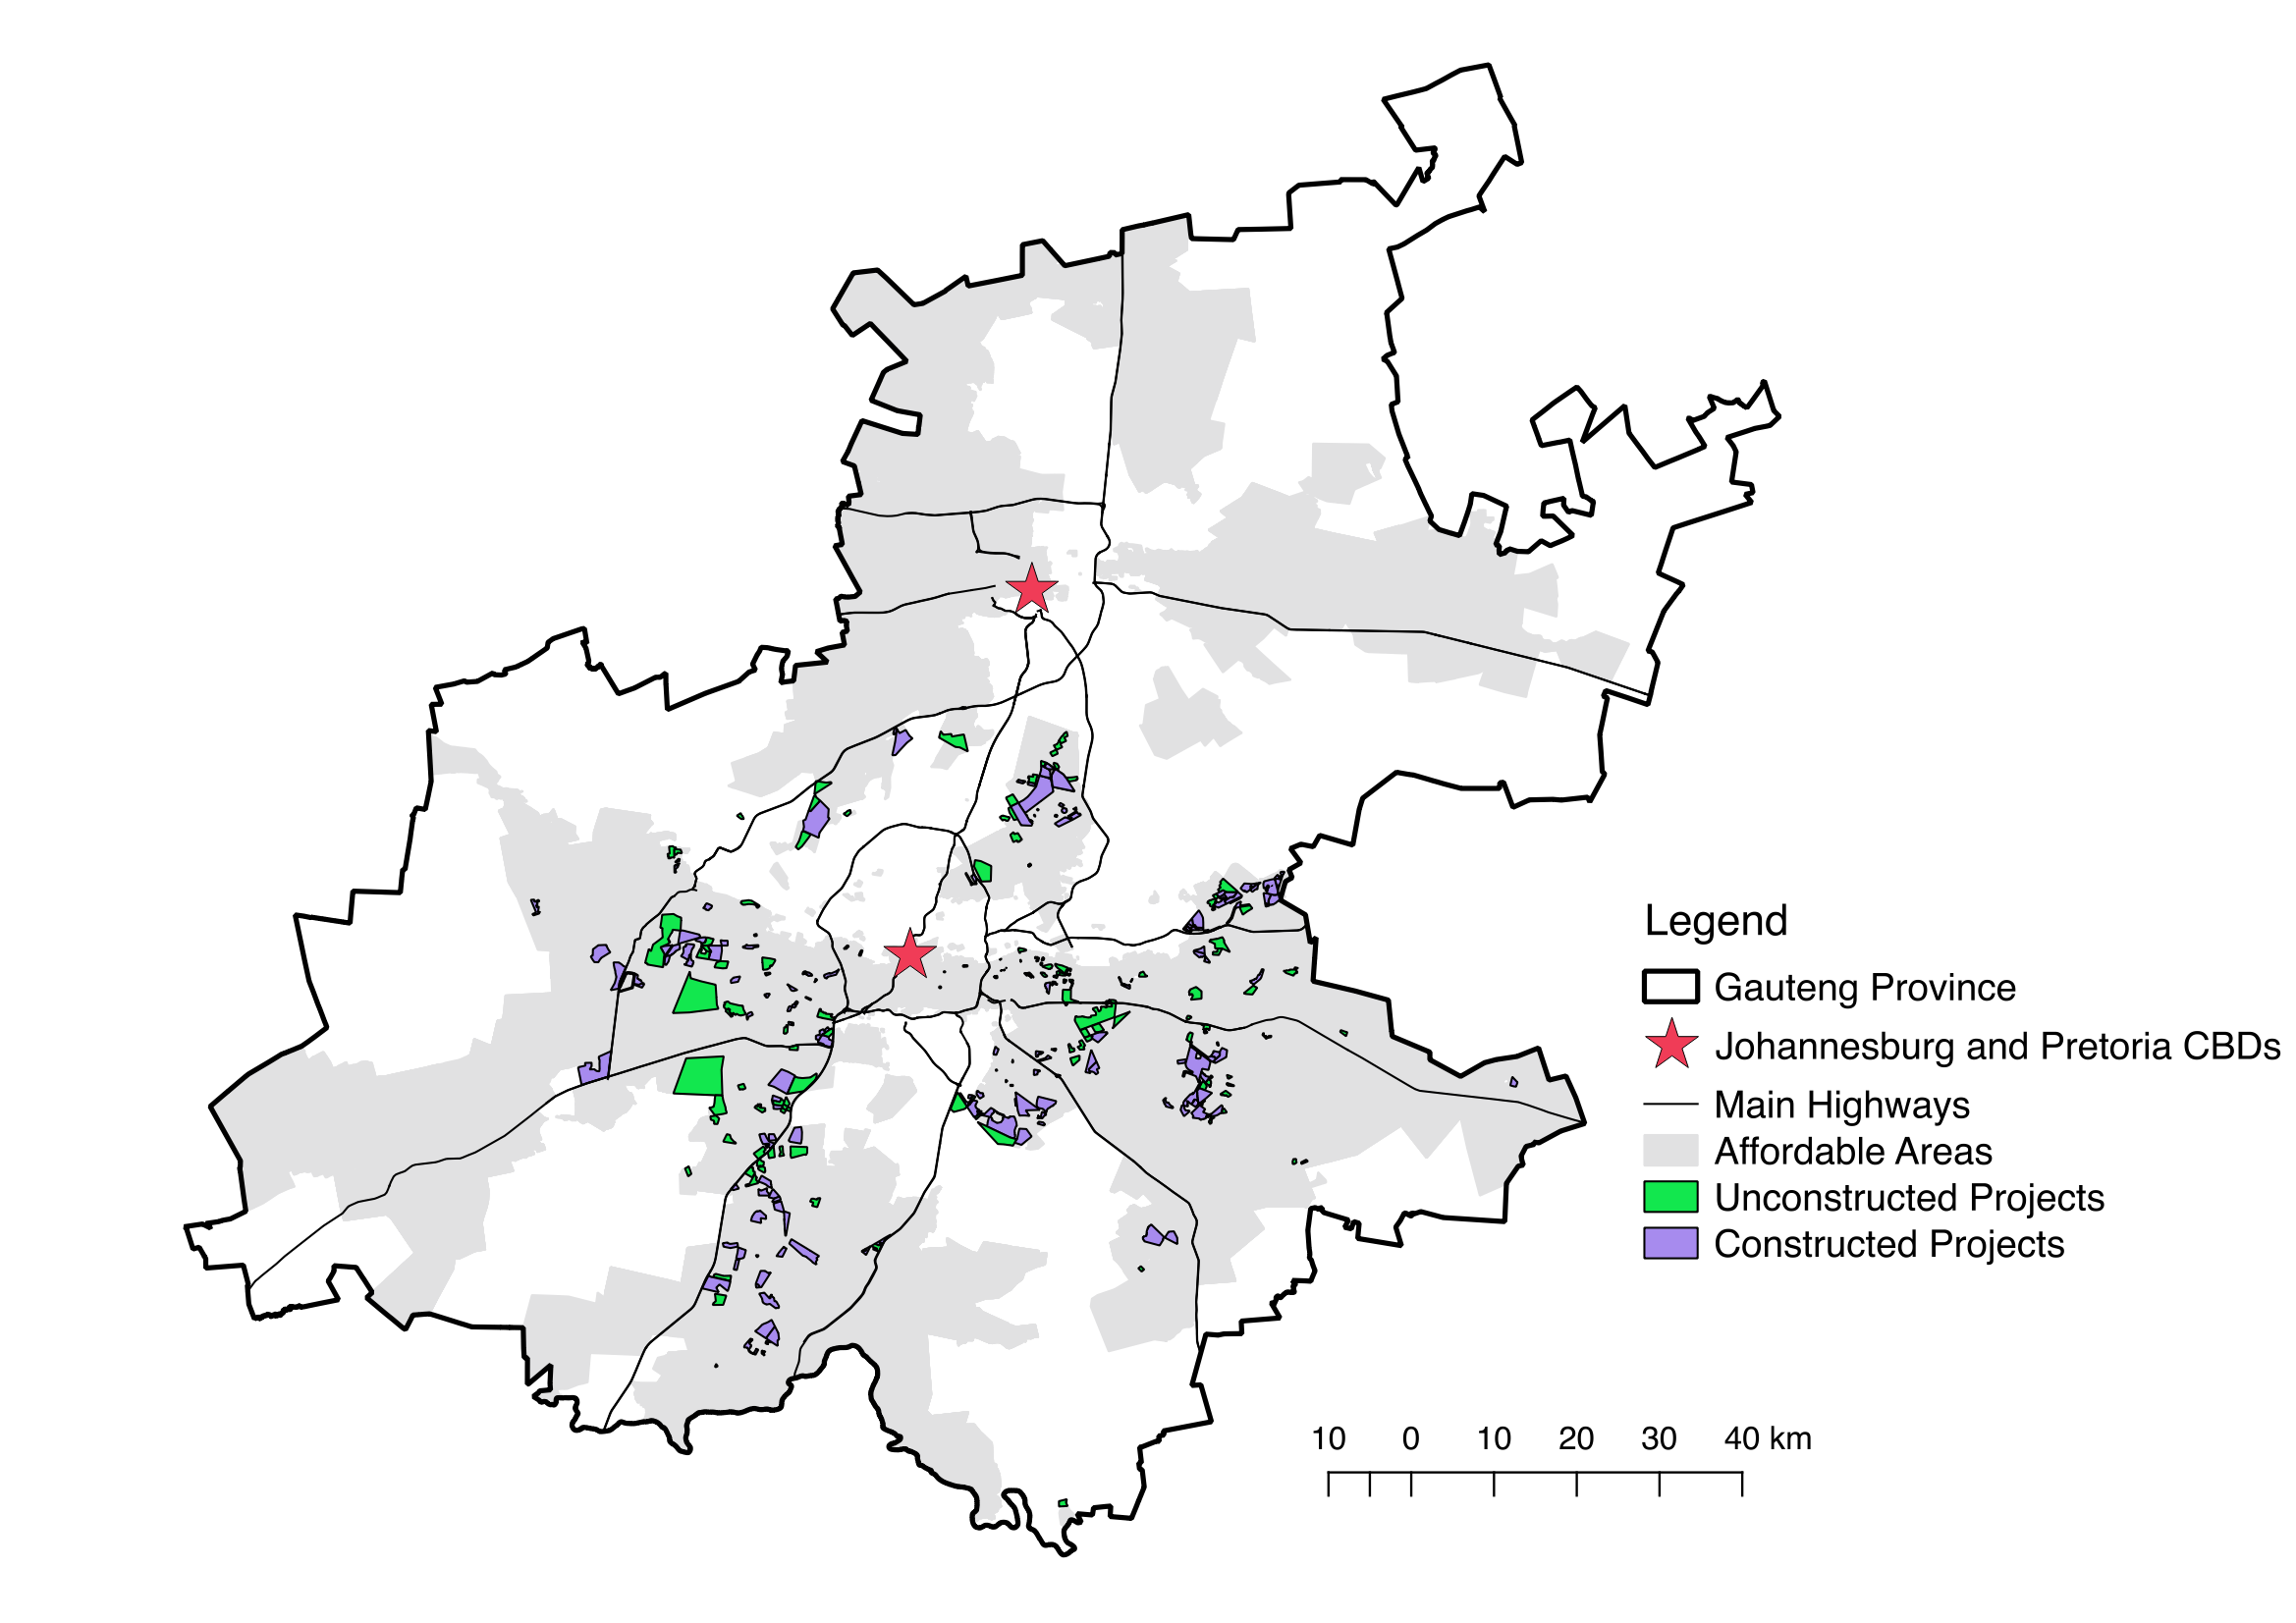
\includegraphics[scale=.6,trim={.9cm .4cm .9cm .4cm}]{figures/projmap_1.png}}
\end{figure}

Figure \ref{figure:map} maps the sample of constructed and unconstructed projects within the Gauteng province.  Projects are generally located far from central business districts, suggesting that inexpensive land plots are targeted by housing authorities.  Outside of the central business district, projects are distributed relatively evenly throughout the Johannesburg metro area.  Despite their distances from Central Business Districts, projects are often next to arterial highways, potentially easing commuting costs for recipients.  Many constructed and unconstructed projects are adjacent to each other while others remain isolated.  

%   Since project construction often occurs in phases, 
%  which is consistent with revisions in project planning and 

% Since project construction often occurs in phases, adjacent constructed and unconstructed projects may indicate partial project completion.  In many other cases, constructed and unconstructed projects are isolated from each other.
% In some cases, constructed and unconstructed projects are adjacent to each other, possibly indicating authorities were unable to complete different phases of planned projects, In other cases, isolated projects of both types.  

% We note that our approach is not without limitations, and may introduce measurement error insofar as we are misattributing deeds to housing projects (false-positives), or assuming a project is unconstructed when it was actually constructed (false-negatives).  

% To provide some validation for our classification, we tabulate in Table~\ref{table:projectdescriptions} project descriptions from the 2008 administrative policy maps according to whether projects are classified as constructed or unconstructed by 2011.  As of 2008, we find that constructed projects are more likely to be classified as ``completed" or ``under implementation", while unconstructed projects are more likely to fall into ``proposed'' or ``planning'' categories.  Among constructed projects, we find 5 ``proposed'' and 8 ``planning'' indicators, which could imply either (1) these projects are false-positives or (2) while planned at some point prior to 2008, these projects were eventually completed by 2011.\footnote{We are unable to assess the frequency at which these descriptions are updated in the data.}  We also identify a single ``complete'' project as unconstructed, likely because its houses do not appear in our deeds records.  Figure \ref{fig:forchange} in section \ref{section:descriptives} further validates our sample, showing how formal housing increases disproportionately in projects classified as constructed. 


% According to the 1997 Housing Act, the South African Government defines adequate ``housing development'' as (1) ``permanent residential structures with secure tenure, ensuring internal and external privacy and providing adequate protection against the elements'' and (2) ``potable water, adequate sanitary facilities and domestic energy supply'' (\cite{housingact}).  

% To measure the spatial impacts of housing projects, we overlay 10 hm by 10 hm grids on all areas within 40 hm of housing projects.

To measure spatial impacts of housing projects similarly across multiple data sources, we overlay square hectare plots of land (10,000 square meters or 1 square hectometer ``hm'') across all land within 4 km of projects.  We exclude plots where development is infeasible because they intersect with rivers, lakes, and/or mining excavation areas (10\% of total plots), which results in a total of 435,889 plots.  We then measure all spatial outcomes at the plot level.

We measure local physical development by counting the number of houses, businesses, and public service buildings in each plot in 2001 and 2012.  We use hand-coded building data from 2001 and 2012 derived from high-resolution aerial and satellite imagery obtained through a partnership with GeoTerraImage (Pty) ltd., a local remote-sensing specialist.\footnote{\href{http://www.geoterraimage.com/}{\tt http://www.geoterraimage.com/}} The data classify buildings into 30 categories, including formal and informal houses. Informal houses are easily identified from their temporary nature, often made of materials such as recycled wood and corrugated metal. In contrast, formal houses are permanent, generally made out of brick and may have a pitched or a flat roof with tiles, zinc panels, or other materials.\footnote{As a validation exercise, we find high correlations ($\geq$0.85) between formal and informal house counts and similar counts in census data from 2001 and 2011.}  The data also distinguish between non-backyard and backyard informal houses, which are often constructed on the same land plots as formal houses.  Beyond houses, we observe schools, health centers, water utility buildings, electricity buildings, and both formal and informal businesses.  
% We construct outcome variables by counting the number of each type of building in each plot and year.


  % total houses split between formal houses and (3) informal residential structures, which we further decompose into backyard informal and non-backyard informal structures.  
% In Figure \ref{fig:bblumaps}, we provide an example of the raw data and a depiction of our griding procedure, using the 2012 data wave.

We measure demographic and housing characteristics with 2001 and 2011 Censuses of Population and Housing.  We average housing characteristics across households and demographic characteristics across people in each census block and year.  Gauteng is divided between 11,000 blocks in 2001 and 17,000 blocks in 2011, each containing 170 households on average.  We then attribute average census characteristics to each plot according to the census block with the greatest area of overlap.  We are able to match 355,721 plots to blocks in 2001 and 345,674 plots to blocks in 2011.

To examine how projects affect nearby housing prices, we analyze deeds data covering the universe of housing transactions from 2001 to 2011 in ``affordable areas,'' which are defined as census enumeration areas with 2010 mean house prices below R500,000.\footnote{These data were provided by the Affordable Land and Housing Data Centre, which tracks affordable housing markets.}  According to Figure~\ref{figure:map}, affordable areas contain nearly every project boundary.  Deeds include price, property location, property size, buyer name, and seller name.  Within project footprints, we find patterns consistent with the allocation of project houses to recipients: large numbers of properties are transferred in the same year at identical, low prices from sellers that are likely to be government housing authorities.\footnote{On average, constructed project footprints contain 316 transactions with seller names that contain ``government,'' ``municipality,'' ``city,'' or ``housing authority'' while unconstructed project footprints contain just 14.}  Since we are unable to precisely distinguish private sellers from government housing authorities within project footprints, we focus on property transactions that are located outside of project areas and are not sold by sellers with more than 30 transactions or whose names include ``government,'' ``municipality,'' ``city,'' or ``housing authority.''  We also exclude the top 1\% of prices as well as prices below 2,500 Rand, which are likely to be composed of mismeasured prices or titles exchanged between family members.  Following these criteria, our sample includes 247,131 deeds from 0 to 40 hm from housing project footprints.  

We attribute properties to plots according to the greatest area of overlap.  To match building and census observations from 2001 and 2011, we calculate average prices and number of transactions in each plot separately for transactions before 2006 (covering 21,330 plots) and after 2006 (covering 18,846 plots).  We also calculate averages for transactions before 2004 and after 2009, which may more closely reflect conditions in 2001 and 2011 respectively although reducing the sample size of transactions.







% We focus on properties located within 1.5 kilometers of constructed and unconstructed housing projects, forming a sample of over 62,000 transactions.  

% The deeds cover the universe of housing transactions from 2001 to 2011 in ``affordable areas,'' which are defined as census enumeration areas with 2010 mean house prices below R500,000.\footnote{These data were provided by the Affordable Land and Housing Data Centre, which tracks affordable housing markets.} Deeds include price, GPS location, plot size, buyer name, and seller name.  


% Although the data do not identify whether deeds belong to housing projects, we are able to infer project status according to whether the seller name includes a government or municipality when first transacted.  This project definition also excludes deeds flagged as large buildings used for commercial purposes (less than 2\% of transactions) as well as purchase prices more than R50,000 above the yearly nominal subsidy values (less than 4\% of remaining transactions), resulting in a sample of over 48,000 deeds.  Appendix Figure \ref{figure:transactionhist} plots the histogram of sale prices according to this project definition, finding substantial bunching around subsidy values for project deeds and a smooth distribution for non-project deeds.  We assign a completion date according to the modal year and month for deeds within each project.  Within projects, most government-sponsored properties are transacted in the same month.\footnote{Appendix \ref{appendix:histfreq} plots the distribution of subsidized and non-subsidized transactions around the modal transaction month.} 

% Though we observe responses from every surveyed household in both census waves, the data does not allow for linking households across time periods. 

% We analyze household-level responses describing the quality of their living quarters. 
% Our outcomes are mainly binary indicators and pertain to the household's access to services (flush toilets, water tap, electricity access), housing durability, and tenure arrangements. 
% We identify households 

% \subsection{Building Based Land Use}
% \label{section:data:bblu}



\section{Descriptive Statistics for Project Neighborhoods at Baseline}\label{section:descriptives}


We provide descriptive evidence on project areas at baseline (before project construction) in Table~\ref{table:projectdescriptives} in order to characterize which types of areas receive constructed and unconstructed projects.

Housing projects are located on less developed land plots (``inside'') within more developed neighborhoods (``0 - 10 hm'') compared to areas further from housing projects (``20 - 40 hm'') across measures of housing quality, public services, and infrastructure access.\footnote{\hmref}  These findings match qualitative evidence that policymakers prioritize locating projects on low-cost land nearby employment opportunities \citep{beninterview}.

Areas inside constructed projects have higher densities of formal housing and much higher densities of informal housing as well as people than areas inside unconstructed projects, which is consistent with anecdotal evidence that policymakers prioritize some areas with dense preexisting slums for housing project implementation \citep{hofmeyr2008risk}.  Higher densities of formal housing in constructed project areas may indicate that parts of housing projects may have already been completed by 2001.  Constructed and unconstructed experience similar levels of infrastructure access and home quality (electric lighting, flush toilets, and piped water inside).  

Areas nearby projects (0 - 40 hm) are more similar between constructed and unconstructed projects than areas within projects.  This finding may be partially driven by the fact that constructed and unconstructed projects are often clustered nearby each other as indicated in Figure~\ref{figure:map}.



% Table~\ref{table:projectdescriptives} compares average attributes for constructed and unconstructed projects.  The first row finds that constructed projects receive 374 deeds houses while unconstructed projects only receive 11 deeds houses on average from 2001 to 2011.  Since deeds houses provide an independent measure of project construction, this finding suggests that few unconstructed projects are misclassified as constructed projects.  Housing prices within 1 km of both constructed and unconstructed projects are lower than for areas over 1 km from projects, indicating that housing authorities locate projects in neighborhoods with inexpensive land.  Size, timing, location, and nearby house prices are broadly similar between unconstructed and constructed projects.  Housing projects cover over 1 $\text{km}^{2}$, which represents a significant development in local neighborhoods.  Using census data, Appendix Table \ref{table:projectdescriptivescensus} finds that before project construction, houses in project footprints are smaller and have worse access to services compared to other houses.  




% All other attributes of housing 
%  the location, size, and surrounding housing stock of the 317constructed and unconstructed projects.  shows that constructed projects deliver an average of 374 houses as measured by the deeds data.  By contrast, projects flagged as unconstructed only produce 11 houses on average, suggesting that 
% validated also by the descriptive changes in housing projects... 
% Constructed projects are also substantially larger in area than unconstructed projects. these discrepancies may be due to many unconstructed projects representing smaller planned extensions to previously implemented projects. 
% It may also reflect the fact that larger land plots are first targeted by housing authorities to maximize delivery. 
% Though unconstructed projects are located in slightly more remote locations, both types of projects impose long commutes on residents, as measured by the average distance to central business districts. 
% These distances are consistent with housing authorities targeting inexpensive, vacant land for these projects. Finally, prices for non-subsidized housing in the vicinity of project boundaries are slightly lower for unconstructed projects, perhaps driven in part by their more distant locations.

% \vspace{0mm}
% \begin{table}[h!]
% \centering
% \caption{Housing Project Areas Description}\label{table:projectdescriptives}
% \vspace{0mm}
% \begin{tabular}{l*{1}{cc}}
% \toprule
%   &Constructed & Unconstructed \\
% \midrule
%  Deeds project houses  & 374  & 11  \\ 
 Median construction year  & 2006  & 2006  \\ 
 Area ($\text{km}^{2}$)  & 1.17  & 1.16  \\ 
 House prices within 1 km (Rands$^\dagger$)  & 188,441  & 218,635  \\ 
 Distance to CBD$^\ddagger$ (km)  & 32.5  & 27.7  \\ 
 Number of Projects  & 172  & 145  \\ 

% \bottomrule
% %\multicolumn{3}{l}{\scriptsize Const. refers to constructed projects and unconst. refers to unconstructed projects.}\\[-.5em]
% %\multicolumn{3}{l}{\scriptsize $^*$Calculated from {\it expected} completion dates using Gauteng National Treasury budget reports.}\\[-.5em]
% \multicolumn{3}{l}{\scriptsize $^\dagger$ The USD averaged around 7.70 Rands during the 2001-2011 period.}\\[-.5em]
% \multicolumn{3}{l}{\scriptsize $^\ddagger$Measured with respect to Johannesburg and Pretoria CBDs. } \\[-.5em]
% \end{tabular}
% \end{table} 



\vspace{0mm}
\begin{table}[h!]
\centering
\caption{Average Characteristics per Plot before Project Construction}\label{table:projectdescriptives}
\vspace{0mm}
\resizebox{1\linewidth}{!}{
\begin{threeparttable}
\begin{tabular}{l*{1}{rrrrrr}}
\toprule
\\[-.5em]
&\multicolumn{3}{c}{Constructed Projects} &\multicolumn{3}{c}{Unconstructed Projects}  \\[.5em] 
Plot location& Inside & 0 - 10 hm  & 20 - 40 hm & Inside & 0 - 10 hm  & 20 - 40 hm \\[.3em]
\\[-.5em]
Buildings \\ \midrule
\\[-.5em]
 \hspace{1em}Formal houses  & 2.28  & 3.96  & 1.35  & 0.61  & 2.77  & 1.67  \\[.15em] 
 \hspace{1em}Informal houses  & 8.86  & 3.20  & 0.57  & 1.93  & 2.72  & 1.08  \\[.15em] 
 \hspace{1em}Health centers  & 0.00  & 0.00  & 0.01  & 0.00  & 0.01  & 0.00  \\[.15em] 
 \hspace{1em}Schools  & 0.04  & 0.06  & 0.02  & 0.01  & 0.04  & 0.03  \\[.15em] 
 \hspace{1em}Shops  & 0.02  & 0.06  & 0.06  & 0.01  & 0.05  & 0.06  \\[.15em] 
 \hspace{1em}Observations  & 15,649  & 64,295  & 347,518  & 13,257  & 64,736  & 351,417  \\[.15em] 

\\[-.5em]
Census Outcomes \\ \midrule
\\[-.5em]
 \hspace{1em}People  & 33.62  & 24.45  & 9.22  & 8.09  & 19.31  & 12.36  \\[.15em] 
 \hspace{1em}Rooms per house  & 2.73  & 3.32  & 3.60  & 2.92  & 3.41  & 3.55  \\[.15em] 
 \hspace{1em}Owns house  & 0.31  & 0.38  & 0.34  & 0.23  & 0.36  & 0.35  \\[.15em] 
 \hspace{1em}Electric lighting  & 0.52  & 0.68  & 0.71  & 0.48  & 0.67  & 0.71  \\[.15em] 
 \hspace{1em}Flush toilet  & 0.58  & 0.71  & 0.70  & 0.50  & 0.70  & 0.71  \\[.15em] 
 \hspace{1em}Piped water inside  & 0.18  & 0.37  & 0.44  & 0.30  & 0.41  & 0.41  \\[.15em] 
 \hspace{1em}Is Employed  & 0.55  & 0.64  & 0.76  & 0.64  & 0.67  & 0.74  \\[.15em] 
 \hspace{1em}Household income (Rand)  & 1,143  & 1,957  & 3,329  & 2,629  & 2,468  & 3,080  \\[.15em] 
 \hspace{1em}Observations  & 15,371  & 60,952  & 271,224  & 11,997  & 60,222  & 277,445  \\[.15em] 

\\[-.5em]
House Prices \\ \midrule
\\[-.5em]
 \hspace{1em}Price (Rand)  &   & 129,840  & 190,598  &   & 165,440  & 173,517  \\[.15em] 
 \hspace{1em}Observations  &   & 6,584  & 14,948  &   & 4,723  & 16,880  \\[.15em] 

\\[-.3em]
 Number of Projects & 166 & 166 & 166 & 140 & 140 & 140 \\[.15em]   Average Project Area ($\text{km}^{2}$) & 1.18 & 1.18 & 1.18 & 1.19 & 1.19 & 1.19  \\[.15em]  
\bottomrule
\end{tabular}
\begin{tablenotes}
\item \footnotesize \hmref Outcomes are measured for 1 hectare plots.  One hectare equals one $\text{hm}^{2}$.  The USD averaged around 7.70 Rands during the 2001-2012 period.  
\end{tablenotes}
\end{threeparttable}
}
\end{table} 




\section{Empirical Methodology}\label{section:methodology}


\begin{figure*}[hbtp]
    \caption{Measuring Spatial Exposure to \\ Example Housing Projects}
    \label{fig:spatialexposure}
    \centering
    \vspace{2mm}
    \begin{subfigure}[b]{.8\textwidth}
        \centering
        \caption[]{\small Plots overlapping with projects}  
        \vspace{-1mm}
        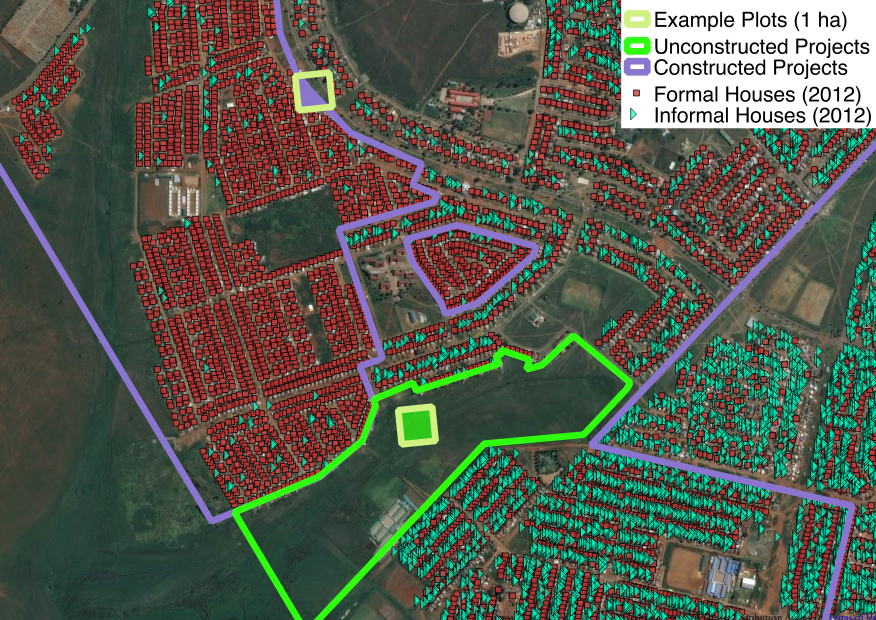
\includegraphics[width=\textwidth,trim={.2cm .2cm .2cm 0cm}, clip=true]{figures/hm_proj_75.png}
        \label{fig:insideproj}
    \end{subfigure}
    \vskip 1mm \vskip 0pt
    \begin{subfigure}[b]{.8\textwidth}  
        \centering 
        \caption[]{\small Plots outside of projects}
        \vspace{-1mm}
        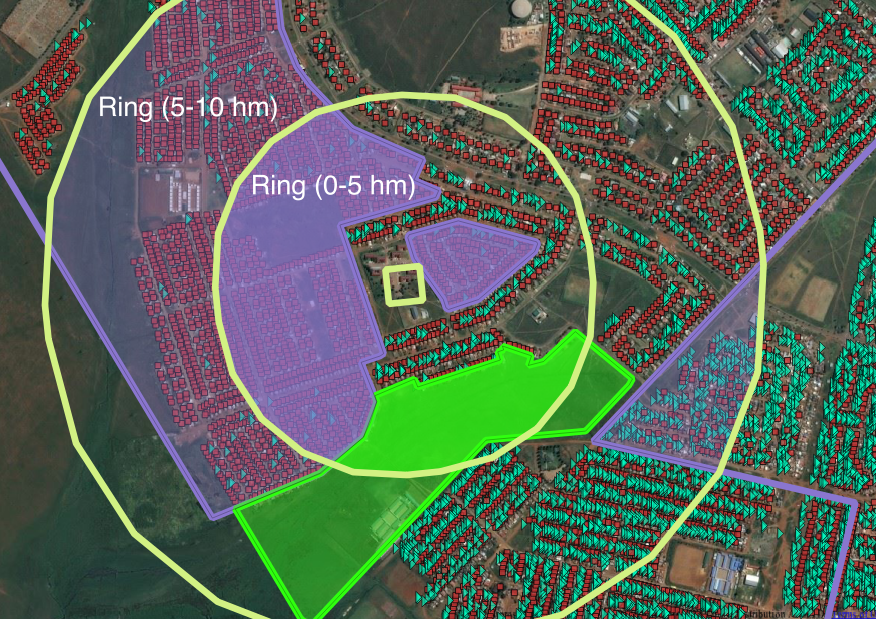
\includegraphics[width=\textwidth,trim={.2cm .2cm .2cm 0cm}, clip=true]{figures/hm_spill_75.png}
        \label{fig:outsideproj}
    \end{subfigure}\\
    {\footnotesize \hmrefha}
\end{figure*} 



\begin{table}
\small
\centering
\caption{Spatial Exposure Summary Statistics}\label{table:spatialsummary}
\vspace{-2mm}
% \resizebox{1\linewidth}{!}{
\begin{threeparttable}
\begin{tabular}{lGG}
\toprule
& Constructed Project Overlap (ha) & Unconstructed  Project Overlap (ha) \\
\midrule
\\[-.7em]
 \hspace{2em}Plots   & 1.000  & 0.046  & 0.038  \\[.15em] 

\\[-.5em]
\hspace{2em}Rings around plots (hm)   \\
 \hspace{3em} 0 - 5   & 98.504  & 0.914  & 0.773  \\[.15em] 
 \hspace{3em} 5 - 10   & 255.512  & 4.919  & 4.086  \\[.15em] 
 \hspace{3em} 10 - 15   & 412.520  & 10.703  & 8.620  \\[.15em] 
 \hspace{3em} 15 - 20   & 569.528  & 17.255  & 13.679  \\[.15em] 
 \hspace{3em} 20 - 25   & 726.535  & 24.009  & 18.930  \\[.15em] 
 \hspace{3em} 25 - 30   & 883.543  & 30.909  & 24.432  \\[.15em] 
 \hspace{3em} 30 - 35   & 1,040.551  & 37.837  & 30.288  \\[.15em] 
 \hspace{3em} 35 - 40   & 1,197.559  & 44.720  & 36.212  \\[.15em] 

\bottomrule
\end{tabular}
\begin{tablenotes}
\item \footnotesize \hmrefha Sample includes plots within 40 hm of projects.  Overlap for rings around plots is only measured for plots outside of projects.
\end{tablenotes}
\end{threeparttable}
% }
\end{table}



To estimate project impacts, we compare changes in outcomes between constructed projects and planned but unconstructed projects.  We estimate both direct effects inside project footprints as well as spillover effects nearby project footprints.  To examine these effects when projects are clustered together and vary in size, we develop a new measure of spatial exposure to place-based policies according to the extent to which each land plot's footprint and immediate neighborhoods overlap with project footprints.  

For plots that overlap with project footprints, we measure direct exposure in terms of how much of each plot's area overlaps with project footprints, which can be expressed as $\text{Area}\big(\textsc{Plot}  \cap  \textsc{Proj.}\big)$.  Figure~\ref{fig:insideproj} includes an example plot that overlaps with a constructed project (upper) as well as an example plot that overlaps with an unconstructed project (lower).  Since the upper plot only partially overlaps with a constructed project, its exposure lies between 0 and 1 ha.\footnote{\haref}  The lower plot falls completely within an unconstructed project indicating exposure equal to 1 ha.  On average across all plots, overlap between plots and projects equals 0.046 ha for constructed projects and 0.038 ha for unconstructed projects. Table~\ref{table:spatialsummary} summarizes this measure.

For plots that do not overlap with project footprints, we measure spillover exposure by first, constructing 5 hm rings around each plot and second, calculating how much of each ring's area overlaps with project footprints, which can be expressed as $\text{Area}\big(\textsc{Ring}  \cap  \textsc{Proj.}\big)$.\footnote{\hmref}  Figure~\ref{fig:outsideproj} provides an example plot that falls just outside of project footprints but whose neighborhood rings from 0 to 5 hm and from 5 to 10 hm overlap with both constructed and unconstructed projects.  Table~\ref{table:spatialsummary} summarizes these measures across neighborhood rings and constructed and unconstructed projects.  We find that exposure increases with the radius of rings growing from 0.9 ha for 0 to 5 hm rings up to 44.7 ha for 35 to 40 hm rings for constructed projects.  

Compared to the standard approach of measuring exposure in terms of the distance to the nearest project,\footnote{See \cite{diamond2016wants}, \cite{rossi2010housing}, and \cite{neumark2015place} for examples of the standard approach.} spatial overlap may better account for variation in the size, shape, and orientation of projects relative to each other.  For example, a plot surrounded by many large projects may develop differently from a plot near one small project although both plots may share the same distance to their nearest project.  The map of projects in Figure~\ref{figure:map} indicates substantial variation in the layout of housing projects across space.  This exposure measure also places greater weight on projects that cover larger land areas, which are also likely to reflect both larger government investments and larger changes to local neighborhoods.

This approach nests the intuition that housing projects may affect local economic outcomes by shifting neighborhood amenity values through changes in housing quality, composition of neighbors, and infrastructure quality.  In this setting, larger projects may produce greater shifts in these amenities, which in turn drive greater incentives to invest in these neighborhoods.  This approach may be less appropriate for place-based policies where households care mainly about their closest access point such as for schools or hospitals.  

Given these measures, we construct an estimating equation of the following form
\begin{align}
\label{eq:main}
\begin{split}
\quad y_{it}  =\,&\mathbbm{1}\Big\{\text{Area}\big(\textsc{Plot}_i  \cap  \textsc{Proj.}\big)>0\Big \}\,\times \Bigg[ \, ( \alpha_0 \, +  \, \alpha_1 \textsc{\small Post}_{t}) \, \times \, \text{Area}\big(\textsc{Plot}_i  \cap  \textsc{Proj.}\big) \, + \\[.5em]
&\hspace{14.5em}( \alpha_2 \, +  \, \alpha_3 \textsc{\small Post}_{t})  \, \times \, \text{Area}\big(\textsc{Plot}_i \cap \textsc{Con. Proj.}\big)\, \Bigg] \, + \\[.7em]
&\mathbbm{1}\Big\{\text{Area}\big(\textsc{Plot}_i  \cap  \textsc{Proj.}\big)=0\Big \}\,\times \Bigg[ \, \sum_{k=1}^{K} \, (\beta_{0}^{k} \,+\, \beta_{1}^{k} \textsc{\small Post}_{t})  \, \times \, \text{Area}\big(\textsc{Ring}_i^{k}  \cap  \textsc{Proj.}\big) \, + \\[.5em]
&\hspace{16.2em}(\beta_{2}^{k} \,+\, \beta_{3}^{k} \textsc{\small Post}_{t})  \, \times \,\text{Area}\big(\textsc{Ring}_i^{k}  \cap \textsc{Con. Proj.}\big)\, \Bigg]  +  \\[.5em]
&\gamma_0 \,+\, \gamma_1 \, \textsc{Post}_t + \varepsilon_{it}
\end{split}
\end{align}

\noindent $y_{it}$ is the outcome for plot $i$ observed at time $t$.  $\textsc{Post}_{t}$ equals one after scheduled construction and zero otherwise.  $\text{Area}\big(\textsc{Plot}_i  \cap  \textsc{Proj.}\big)$ measures the area of overlap between plot $i$ and all project footprints while $\text{Area}\big(\textsc{Plot}_i \cap \textsc{Con. Proj.}\big)$ measures the hectares of overlap between plot $i$ and only project footprints that are successfully constructed.  Likewise, $\text{Area}\big(\textsc{Ring}_i^{k}  \cap  \textsc{Proj.}\big)$ measures the  hectares of overlap between a ring from $5(k-1)$ to $5k$ hm around plot $i$ and all project footprints.   $\text{Area}\big(\textsc{Ring}_i^{k}  \cap  \textsc{Proj. Con.}\big)$ measures the hectares of overlap for this ring and only project footprints that are successfully constructed.  We consider concentric 5 hm rings ranging from 0 to 40 hm away from plots that implicitly assumes that any spillover effects dissipate by 40 hm, which is consistent with recent literature on place-based policies.\footnote{\cite{diamond2016wants} and \cite{rossi2010housing} find that main effects are concentrated within 10 hm of place-based policies.}  For reference, Figure~\ref{fig:spatialexposure} includes an example of rings from 0 to 5 hm and 5 to 10 hm.  $\gamma_0$ includes a constant term, $\gamma_1$ controls for average changes in outcomes in the post period, and $\varepsilon_{ipt}$ is the idiosyncratic error term.  Standard errors are clustered at the project-level with projects assigned to each plot according to the greatest area of overlap either with the plot's footprint or with the closest overlapping ring.  

For plots that overlap with project footprints (ie. $\text{Area}\big(\textsc{Plot}_i  \cap  \textsc{Proj.}\big)>0$), we estimate the direct effects of project construction.  Our coefficient of interest, $\alpha_3$, measures the change in outcomes for plots overlapping with constructed projects relative to plots overlapping with planned but unconstructed projects.  Likewise, for plots outside of project footprints (ie. $\text{Area}\big(\textsc{Plot}_i  \cap  \textsc{Proj.}\big)>0$), we estimate the spillover effects of project construction.  Each coefficient of interest, $\beta_3^{k}$, measures the differential change in outcomes for plots whose neighborhoods from $5(k-1)$ to $5k$ hm overlap with constructed project footprints relative to plots whose neighborhoods overlap with unconstructed project footprints by hectares of overlap.  These coefficients capture the causal effects of project construction under the assumption that in the absence of project construction, plots exposed to constructed project footprints would have evolved in the same way as plots exposed to unconstructed project footprints.  We do not estimate spillover effects for plots within project footprints because spillover effects for these plots would be mainly identified from the relative locations of plots within project footprints (ie. near the edge versus in the interior of a footprint) and these relative locations within plots are likely to capture variation in where project houses are constructed within footprints instead of the true spillover effects of having greater nearby exposure to projects.

Our flexible specification of spillover effects from 0 to 40 hm allows us to examine how these effects dissipate across space.  We hypothesize that spillover effects are likely to be concentrated in nearby neighborhoods.  This specification also provides a partial test for whether areas with constructed projects and areas with unconstructed projects are likely to follow parallel trends.  We hypothesize that spillover effects are likely to dissipate at further distances (ie. 20 to 40 hm).  Therefore, evidence of effects at these distances may suggest that areas with constructed projects develop differently from areas with unconstructed projects for reasons unrelated to project construction.  For example, housing projects may be accompanied by broader urban renewal programs that affect broader areas around projects.  Alternatively, policymakers may prioritize growing areas for project construction.

By comparing changes over time, this approach accounts for baseline differences between constructed and unconstructed project areas.  This approach also controls for aggregate factors that affect development in the metro-area by examining differential changes between constructed and unconstructed project areas.  

This framework does not allow for trends that are also correlated with whether projects are constructed.  For example, forward-looking households may anticipate project construction and alter their housing investment decisions accordingly.  Qualitative evidence suggests that it would be difficult for households to anticipate construction in this context due to substantial uncertainty in project location and timing.  Project managers face difficulties coordinating stakeholders and sourcing funding while housing authorities are rarely transparent about project planning \citep{serihistory}.\footnote{\cite{diamond2016wants} also leverage uncertainty in project timing to study affordable housing in the US.} 

Our approach assumes that project construction occurs between 2001 and 2012.  To the extent that some parts of projects may have been constructed before 2001, our estimates of the effects of project construction would be biased toward zero, suggesting that our approach may underestimate the full effects.



\section{Estimates of Direct and Spillover Effects}\label{section:results}

% To draw statistical inference on the patterns depicted in section \ref{section:descriptives}, we proceed to estimate variants of equation (\ref{eq:main}) for each outcome of interest. 

% Backyard housing is a common phenomenon in South Africa where households erect informal dwellings within the plots of formal dwellings \citep{Brueckner2018backyarding}.  Project houses may be well-suited for backyarding because each house receives an individual landplot that is often much larger than the house itself. put this up top!!  with a discussion of the maps!!

% where the outcomes are housing densities in 25m by 25m plots in 2001 and 2012 measured in terms of houses per $\text{km}^{2}$.  $\textsc{\small Post}_{t}$ indicates observations in 2012.  Table~\ref{table:bbluDDDfull} reports the coefficient estimates.

% \footnote{Appendix Table~\ref{table:bbluDDDfull} includes the full set of coefficients as well as additional outcomes.}  Results are reported in terms of houses per $\text{km}^{2}$.  

% To examine how spillover effects dissipate with distance, Figure~\ref{fig:gr_coef} graphs coefficients for hectares of constructed project overlap with 5 hm neighborhood rings from 0 to 40 hm ($\beta_3^{1}$ to $\beta_3^{8}$) for two outcomes: people per hectare and houses per hectare.  Coefficients are statistically significant at the 1\% level and positive for overlap with 0-5 hm rings.  This finding suggests that exposure to housing projects in immediate neighborhoods drives large increases in a plot's population and housing.  Coefficients for rings beyond 5 hm are statistically insignificant and hover around zero, which indicates that spillover effects quickly dissipate at greater distances.  Zero effects for exposure further from projects further suggests that constructed and unconstructed projects are unlikely to experience differential policies or shifts in economic growth that affect all areas evenly within 4 hm of projects, providing some support to our identification assumption of parallel trends in outcomes between constructed and unconstructed projects in the absence of construction.  In the following tables, we report results for the closest ring (0 to 5 hm) while including estimates for all rings in the Appendix.
% The first row of column (1) indicates that overlapping with constructed projects generates an increase in 2,574 people per $\text{km}^{2}$.  Likewise, for plots that do not overlap with projects, the second row indicates that moving from 0 to 100\% overlap of a 0 to .5 km neighborhood with constructed projects generates an increase of 2,103 people per $\text{km}^{2}$.  We calculate the total effect per project by multiplying the coefficients by the total plot footprint and neighborhood exposures per project.  We calculate total footprint exposure per project equal to 1.19, which is also the average size of projects in $\text{km}^{2}$, and total neighborhood exposure per project equal to 0.24.  With this formula, coefficients from Table~\ref{table:main} indicate that projects lead to increases of 3,083 people within their footprints and 512 people in their immediate neighborhoods.  


% Table~\ref{table:main} includes coefficients for the direct effect, $\alpha_3$ and the spillover effect, $\beta_3^{1}$ for the 0 to 5 hm ring.  


We first examine the direct and spillover effects of projects on housing and population by estimating equation (\ref{eq:main}).  We focus on spillover effects for 0 to 5 hm rings because estimates for rings from 5 to 40 hm  are statistically insignificant and hover around zero.\footnote{\hmref}  Appendix Figure~\ref{fig:gr_coef_w_sd} plots coefficients for constructed project overlap with rings from 0 to 40 hm ($\beta_3^{1}$ to $\beta_3^{8}$) for people and houses per hectare.  We report results for the closest ring (0 to 5 hm) while including estimates for all rings in the Appendix.

\begin{table}
\small
\centering
\caption{Population and Housing}\label{table:main}
\vspace{-2mm}
\resizebox{1\linewidth}{!}{
\begin{threeparttable}
\begin{tabular}{lCCCCC}
\toprule
                    &(1)&(2)&(3)&(4)&(5)\\[.5em] &Population Density                   &Total Formal Housing                   &Total Informal Housing                   &Backyard Informal Housing                   &Log(Price) \\ \midrule \\[-.6em]                   \\
\textsc{\% Project Overlap with:} \\[1em] \hspace{1.5em}\textsc{Footprint}&      2573.7\textsuperscript{a}&       663.0\textsuperscript{a}&       247.3\textsuperscript{b}&       664.9\textsuperscript{a}&        -0.1                   \\
                    &     (463.0)                   &      (81.2)                   &     (104.4)                   &     (115.8)                   &       (0.4)                   \\[.5em]
\hspace{1.5em} \textsc{0-.5km Neighborhood }&      2102.9\textsuperscript{a}&       231.4\textsuperscript{b}&       461.2\textsuperscript{b}&       361.2\textsuperscript{a}&         0.4                   \\
                    &     (738.7)                   &     (105.2)                   &     (182.5)                   &     (132.4)                   &       (0.5)                   \\[.5em]
Mean Pre            &     1,342.0                   &       179.8                   &       137.0                   &        52.1                   &        11.6                   \\
Mean Post           &     1,927.2                   &       241.7                   &       239.6                   &       152.1                   &        12.2                   \\
R$^2$               &       0.090                   &       0.081                   &       0.093                   &       0.079                   &       0.126                   \\
N                   &     701,395                   &     871,772                   &     871,772                   &     871,772                   &      41,132                   \\

\bottomrule
\end{tabular}
\begin{tablenotes}
\item \footnotesize Population is from census data and houses are from the building data. \regtext Appendix Table~\ref{table:main_full} includes the full set of coefficients.
\end{tablenotes}
\end{threeparttable}
}
\end{table}


Column (1) of Table~\ref{table:main}  finds a direct effect of 25.7 people per hectare, which is statistically significant at the 1\% level.  Since each plot covers one hectare, this result suggests that plots within constructed project footprints grow by 25.7 people as a result of project construction.  This change represents an almost doubling of the pre-period mean of 13.4 people per hectare.  Since constructed projects on average cover 119 ha, this estimate indicates a population increase per project equal to 3,063 people within project footprints.  This result suggests that constructed housing projects generate large-scale growth in local populations compared to similar but unconstructed project areas.

We also find a spillover effect of 0.21 people per hectare, which is statistically significant at the 1\% level.  The spillover effect is nearly 100 times smaller in magnitude than the direct effect consistent with plot development being more sensitive to conditions in footprints than in neighborhoods.  However, spillover effects reach a much larger number of plots than direct effects.  On average, each project generates around 2,400 ha of overlap with 0 to 5 hm rings around neighboring plots.  Therefore, the spillover effect per project is 504 people, which is around 16\% of the direct effect per project.  This increase in neighborhood population is consistent with constructed projects providing positive amenities that attract new residents nearby.

Column (2) finds a consistent pattern for houses: direct effects imply a statistically significant increase of 9.1 houses per plot, representing a near tripling of the pre-period average of 3.2 houses.  As in Column (1), spillover effects are also statistically significant and two orders of magnitude smaller than direct effects.  The direct effect implies a massive increase of 1083 houses per project while the spillover effect suggests an additional increase of 168 nearby houses per project.  As a reference, the Low Income Housing Tax Credit in the US produces only around 64 housing units per project \citep{diamond2016wants}.

The remaining columns further disaggregate houses into formal houses (3) and informal houses (4), and then further to informal backyard houses (5).  Backyard housing is a common phenomenon in South Africa where households erect informal dwellings within the plots of formal dwellings \citep{Brueckner2018backyarding}.  In project footprints, formal housing growth is over 2.5 times larger than informal housing growth.  Formal housing growth may include both new government project houses as well as new private housing as developers crowd into these areas.  Among informal houses, backyard houses replace non-backyard houses consistent with qualitative evidence that housing authorities cleared preexisting slums before constructing new projects \citep{hofmeyr2008risk}.  In spillover areas, informal housing growth dominates formal housing growth as people quickly crowd into undeveloped land nearby housing projects possibly to enjoy amenities offered by constructed housing projects.

Appendix Table~\ref{table:main_full} includes the full set of coefficients for equation (\ref{eq:main}) with outcomes from  Table~\ref{table:main}.  Spillover coefficients are insignificant for all but one ring beyond 5 hm across all outcomes, motivating our approach of focusing on spillover effects for 0 to 5 hm rings.  Coefficients for the interaction of Post with plot overlap indicate that unconstructed project areas experience positive changes within their footprints even in the absence of project construction, which is consistent with investment crowding into these relatively undeveloped areas.  Yet, changes for unconstructed projects are at least 3 times smaller than for constructed projects, reiterating the substantial size of project investments.  Small and largely insignificant coefficients for the interaction of Post with 0 to 5 hm ring overlap suggest that unconstructed projects are not associated with nearby spillover changes.  

We also examine whether housing projects affect nearby formal housing prices using deeds data.  Since within project footprints, the vast majority of deeds record transfers of subsidy houses from municipalities to individuals rather than transactions between individual buyers and sellers, we are unable to estimate direct effects.  Therefore, we focus on estimating spillover effects by excluding $\alpha$ coefficients from equation (\ref{eq:main}).  Table~\ref{table:prices} provides estimates of spillover effects on the number of transactions per plot (columns (1) and (2)) and the average price of transactions per plot (columns (3) and (4)).  Columns (1) and (3) define periods pre/post construction as pre/post 2006.  In contrast, columns (2) and (4) define pre construction as before 2004 and post construction as after 2009, which may more precisely reflect conditions before and after construction while including fewer observations.  Columns (1) and (2) find small, statistically insignificant impacts of project construction on the number of transactions per plot.  Point estimates suggest that increasing hectares of overlap with constructed projects by a standard deviation (4.64 ha) leads to .0012 increases in transactions per plot in column (1) and .0012 decreases in column (2).  Columns (3) and (4) find small, statistically insignificant positive impacts of project construction on average prices per plot.  Since prices are expressed in log-terms, point estimates approximate the percentage change in transaction prices associated with an additional hectare of overlap with constructed projects.  Point estimates suggest that a standard deviation greater overlap generates price increases of 1.7\% in column (3) and 4.5\% in column (4).  

Positive effects on local prices are consistent with public housing projects providing positive local amenities.  Yet, the statistical insignificance of these results means that we cannot exclude the possibility of zero or even negative effects of projects on local prices.  One reason for these statistically insignificant results may be that deeds records are relatively rare occurring on only 7.6\% of plots.  This finding underscores the difficulty of estimating spillover effects using official deeds records in contexts where housing transactions are unlikely to be officially recorded.

\begin{table}
\small
\centering
\caption{Formal House Transactions and Prices}\label{table:prices}
\vspace{-2mm}
\resizebox{1\linewidth}{!}{
\begin{threeparttable}
\begin{tabular}{lCCCCC}
\toprule
                    &(1)&(2)&(3)&(4)\\[.5em] &Transactions                   &Transactions                   &   Log Price                   &Log Price \\ \midrule \\[-.6em]                   \\
Post $\times$ Constructed project overlap with: \\[1em] \hspace{1.5em}Plot neighborhood (0-5 hm ring)&     0.00026                   &    -0.00026                   &     0.00368                   &     0.00963                   \\
                    &   (0.00125)                   &   (0.00080)                   &   (0.00481)                   &   (0.00821)                   \\[.5em]
Pre: 2001-2006 Post: 2007-2012&  \checkmark                   &                               &  \checkmark                   &                               \\
Pre: 2001-2004 Post: 2009-2012&                               &  \checkmark                   &                               &  \checkmark                   \\
Mean Pre            &        0.11                   &        0.05                   &       11.58                   &       11.24                   \\
Mean Post           &        0.10                   &        0.06                   &       12.21                   &       12.29                   \\
R$^2$               &       0.001                   &       0.000                   &       0.128                   &       0.243                   \\
N                   &     784,448                   &     784,703                   &      40,176                   &      21,382                   \\

\bottomrule
\end{tabular}
\begin{tablenotes}
\item \footnotesize \regtext
\end{tablenotes}
\end{threeparttable}
}
\end{table}





\section{Mechanisms}

We examine three possible mechanism driving the direct and spillover effects of housing projects.  First, projects may influence \textit{neighborhood quality} by changing both the quality of houses and the types of people living in these houses, which may affect investment decisions in nearby areas even if these areas do not directly benefit from the projects.\footnote{See \cite{rossi2010housing} and \cite{diamond2016wants} for examples.}  Second, projects may be accompanied by investments in \textit{public services} accessible to households within and nearby project footprints.  Third, by increasing local population density, projects may generate \textit{agglomeration economies} as businesses grow nearby to both employ and provide goods for the growing population.


\subsection{Neighborhood Quality}

Table~\ref{table:inf_census} provides estimates of project impacts for five measures of house quality.  According to point estimates, overlapping directly with constructed projects only yields .35 additional rooms and an increase in the likelihood of home ownership by 4\%, both of which are statistically insignificant.  These muted responses may be explained by the large increase in informal, backyard housing that accompanies formal project houses since backyard houses are often smaller and rented from plot owners.  We find similarly small, insignificant spillover effects.  

In contrast to rooms and home ownership, access to basic services increases dramatically and statistically significantly in project footprints.  Overlap with a constructed project improves access to services by 12 percentage points for electric lighting, 24 percentage points for flush toilets, and 28 percentage points for piped water inside the home.  Although spillover effects are similarly positive, their magnitudes are very small and statistically insignificant, indicating little possibility that neighboring houses benefit directly from these services.  

\begin{table}
\small
\centering
\caption{House Quality}\label{table:inf_census}
\vspace{-2mm}
\resizebox{1\linewidth}{!}{
\begin{threeparttable}
\begin{tabular}{lCCCCC}
\toprule
                    &(1)&(2)&(3)&(4)&(5)\\[.5em] &Total Rooms                   &   Own House                   &Electric Lighting                   &Flush Toilet                   &Piped Water Inside\\ \midrule \\[-.6em]                   \\
Post $\times$ Constructed project overlap with: \\[1em] \hspace{1.5em}Plot footprint&      0.3492                   &      0.0396                   &      0.1185\textsuperscript{b}&      0.2367\textsuperscript{a}&      0.2795\textsuperscript{a}\\
                    &    (0.2950)                   &    (0.0535)                   &    (0.0555)                   &    (0.0591)                   &    (0.0550)                   \\[.5em]
\hspace{1.5em}Plot neighborhood (0-5 hm ring)&      0.0044                   &      0.0006                   &      0.0004                   &      0.0008                   &      0.0001                   \\
                    &    (0.0028)                   &    (0.0007)                   &    (0.0009)                   &    (0.0007)                   &    (0.0007)                   \\[.5em]
Mean Pre            &      3.5005                   &      0.3478                   &      0.6921                   &      0.6988                   &      0.4091                   \\
Mean Post           &      3.9838                   &      0.3507                   &      0.7696                   &      0.7515                   &      0.5816                   \\
R$^2$               &       0.063                   &       0.010                   &       0.049                   &       0.034                   &       0.102                   \\
N                   &     698,762                   &     699,801                   &     701,296                   &     701,296                   &     701,296                   \\

\bottomrule
\end{tabular}
\begin{tablenotes}
\item \footnotesize Outcomes are from census data at the household-level. \regtext
\end{tablenotes}
\end{threeparttable}
}
\end{table}

\begin{table}
\small
\centering
\caption{Demographics}\label{table:demo}
\vspace{-2mm}
\resizebox{1\linewidth}{!}{
\begin{threeparttable}
\begin{tabular}{lCCCCC}
\toprule
                    &(1)&(2)&(3)&(4)&(5)\\[.5em] &Age                   &     Married                   &     African                   &Household Size                   &\% Under Age 18 \\ \midrule \\[-.6em]                   \\
Post $\times$ Constructed project overlap with: \\[1em] \hspace{1.5em}Plot footprint&     -0.8989                   &     -0.0222                   &     -0.0233                   &      0.3078\textsuperscript{b}&      0.0236                   \\
                    &    (0.9067)                   &    (0.0175)                   &    (0.0405)                   &    (0.1498)                   &    (0.0172)                   \\[.5em]
\hspace{1.5em}Plot neighborhood (0-5 hm ring)&      0.0041                   &     -0.0001                   &     -0.0006                   &      0.0027\textsuperscript{c}&      0.0001                   \\
                    &    (0.0097)                   &    (0.0002)                   &    (0.0004)                   &    (0.0015)                   &    (0.0003)                   \\[.5em]
Mean Pre            &     41.5897                   &      0.3079                   &      0.7071                   &      3.0403                   &      0.3018                   \\
Mean Post           &     42.5959                   &      0.2981                   &      0.7105                   &      2.7759                   &      0.2665                   \\
R$^2$               &       0.031                   &       0.075                   &       0.111                   &       0.059                   &       0.079                   \\
N                   &     699,656                   &     760,314                   &     760,314                   &     700,795                   &     700,795                   \\

\bottomrule
\end{tabular}
\begin{tablenotes}
\item \footnotesize Outcomes are from census data.  ``Age,'' ``Married,'' and ``African'' are at the person-level while ``Household size'' and ``\% Under Age 18'' are at the household level.  ``Married'' includes only adults over 18.  \regtext
\end{tablenotes}
\end{threeparttable}
}
\end{table}

Table~\ref{table:demo} performs the corresponding exercise for plot demographics.  Point estimates indicate that as a result of project construction, plots that overlap directly with projects are more likely to house younger, unmarried, non-Africans with larger households and more children.  Estimates are statistically insignificant except for the coefficient on household size.  Spillover effects largely mirror direct effects in both relative sizes and statistical significance.  These results provide suggestive evidence that larger households with children either benefit directly from project houses (consistent with projects giving priority to families with children) or move to project areas possibly so that their children enjoy access to basic services.

Taken together, these results are broadly supportive of improvements in neighborhood quality by increasing the availability of basic services as well as attracting younger families nearby (to the extent that these families are perceived as desirable neighbors).  Moreover, large observed increases in backyard shacks are not enough to generate decreases in average room size, home ownership, or access to basic services.


\subsection{Public Services}

Building data allow us to track local investments in public services that may not be directly reflected in census data.  Table~\ref{table:inf_bblu} estimates effects for structures categorized as water utility buildings, electricity utility buildings, health centers, and schools.  We estimate positive direct effects across all categories and coefficients are economically large and statistically significant for all but electricity utility buildings.  For example, plots with constructed project footprints receive .025 more water utility buildings on average, which represents a 227\% increase on the pre-period mean of .01 water utility buildings per plot.  Likewise, health centers and schools increase by more than double their pre-period means.  These results are consistent with public housing projects being complementary with other public goods investments, either directly as part of the projects or indirectly as follow-up investments from local governments.  Although spillover effects are only positive and statistically significant for schools, nearby plots may also benefit from public services in nearby project areas both in terms of service quality (ie. water pressure) and accessibility (ie. distance to health center).  

\begin{table}
\small
\centering
\caption{Public Service Buildings}\label{table:inf_bblu}
\vspace{-2mm}
\resizebox{1\linewidth}{!}{
\begin{threeparttable}
\begin{tabular}{lCCCCCC}
\toprule
                    &(1)&(2)&(3)&(4)\\[.5em] &Water Utility Buildings                   &Electricity Utility Buildings                   &Health Centers                   &Schools \\ \midrule \\[-.6em]                   \\
Post $\times$ Constructed project overlap with: \\[1em] \hspace{1.5em}Plot footprint&     0.02453\textsuperscript{a}&     0.00062                   &     0.00109\textsuperscript{b}&     0.06251\textsuperscript{a}\\
                    &   (0.00532)                   &   (0.00052)                   &   (0.00048)                   &   (0.01455)                   \\[.5em]
\hspace{1.5em}Plot neighborhood (0-.5 km ring)&     0.00005                   &     0.00008                   &    -0.00028                   &     0.00119\textsuperscript{c}\\
                    &   (0.00023)                   &   (0.00006)                   &   (0.00018)                   &   (0.00071)                   \\[.5em]
Mean Pre            &     0.01068                   &     0.00384                   &     0.00525                   &     0.02824                   \\
Mean Post           &     0.01602                   &     0.00481                   &     0.00595                   &     0.04212                   \\
R$^2$               &       0.002                   &       0.000                   &       0.001                   &       0.003                   \\
N                   &     871,778                   &     871,778                   &     871,778                   &     871,778                   \\

\bottomrule
\end{tabular}
\begin{tablenotes}
\item \footnotesize Outcomes are from the building data. \regtext
\end{tablenotes}
\end{threeparttable}
}
\end{table}


\subsection{Agglomeration Economies}

To test whether housing and population increases invite new business and employment, we combine building data on businesses with census data on employment and household income.  Table~\ref{table:agglom} documents large statistically significant increases in businesses within project footprints, amounting to an almost doubling of the pre-period average number of businesses per plot.  Column (2) attributes the majority of this growth to smaller, informal businesses.  Point estimates indicate a 4.8 percentage point increase in employment and a 1.9\% increase in household income although both are statistically insignificant.  Spillover effects across all outcomes are small and statistically insignificant.  While households nearby projects do not appear to experience income or business gains in their plots, these households may still benefit as consumers from new businesses nearby.


\begin{table}
\small
\centering
\caption{Economic Outcomes}\label{table:agglom}
\vspace{-2mm}
\resizebox{1\linewidth}{!}{
\begin{threeparttable}
\begin{tabular}{lCCCC}
\toprule
                    &(1)&(2)&(3)&(4)\\[.5em] &Businesses                   &Informal Businesses                   &Household Employment                   &Log Household Income\\ \midrule \\[-.6em]                   \\
Post $\times$ Constructed project overlap with: \\[1em] \hspace{1.5em}Plot footprint&     0.05333\textsuperscript{a}&     0.03445\textsuperscript{a}&     0.03009                   &     0.01943                   \\
                    &   (0.01263)                   &   (0.00831)                   &   (0.03495)                   &   (0.17251)                   \\[.5em]
\hspace{1.5em}Plot neighborhood (0-.5 km ring)&     0.00042                   &     0.00043                   &     0.00020                   &    -0.00082                   \\
                    &   (0.00039)                   &   (0.00029)                   &   (0.00044)                   &   (0.00153)                   \\[.5em]
Mean Pre            &     0.05584                   &     0.00237                   &     0.81534                   &     7.30960                   \\
Mean Post           &     0.07351                   &     0.00873                   &     0.86282                   &     8.40645                   \\
R$^2$               &       0.001                   &       0.002                   &       0.149                   &       0.380                   \\
N                   &     871,778                   &     871,778                   &     698,873                   &     699,171                   \\

\bottomrule
\end{tabular}
\begin{tablenotes}
\item \footnotesize Businesses are from the building data.  Income at the household level and employment at the individual level are from the census data.  Employment is calculated for individuals between ages 18 to 65. \regtext
\end{tablenotes}
\end{threeparttable}
}
\end{table}


% Taken together, these results are consistent with housing authorities ensuring that preexisting slum residents are able to benefit from new project houses.  The results are less consistent with the hypothesis that political corruption steers project houses toward wealthier and more politically connected households \citep{seriq}.  




\section{Welfare Impacts}\label{section:theory}

%%% motivate more from a broad welfare perspective

% Compare to Diamond's model! in writing;  mention time periods up front?!
% This model is static where households h
% Households and developers make choices independently each time period, which is consistent with mobile populations of households and high maintenance costs as well as low fixed construction costs per house.  

% In most cases, researchers use price changes to infer welfare impacts.  Instead, since price data does not seem to work well in our setting, we want to see what quantity changes imply for welfare changes.  


In order to approximate the welfare impacts of housing projects, we develop a simple model of residential housing markets that maps observed changes in the quantity of housing into welfare changes.  Our approach uses variation in land steepness to shift construction costs and trace demand for housing.  Under the assumption that projects affect housing markets by changing local amenities and that houses within projects participate in a competitive rental market, we recover the value of local amenities that rationalize observed housing quantities.  Amenities provide a reduced-form method of capturing all aspects that may affect the desirability of living on a particular plot (including neighborhood quality, public services, and agglomeration economies).

% This approach assumes that all households have identical housing demand.
% We assume that housing sectors are independent from each other.
% We assume that housing is continuous.
% We assume that there is a competitive rental market for subsidized houses.
% and map quantity changes into welfare estimates.
% Under the assumption of elastic demand for housing, 

 % We assume that households are identical and have perfectly elastic demand for housing.\footnote{This assumption may be reasonable in a context like South Africa where high levels of unemployment mean that different households face similar strong incentives to locate near employment centers.}

% We assume that developers face a constant marginal cost of building houses and are able to set rents to make households indifferent between renting a house and choosing their outside option.

% We then consider welfare impacts under the assumption that housing projects are acting entirely through an amenity channel.
% We develop a simple model of residential housing markets to capture the welfare effects of local housing projects within their neighborhoods.  This model infers welfare changes not only through changes in rents, but also through changes in the quantities of housing supplied.  

% The distribution of $\upsilon_{hjt}$ may be correlated across housing sectors to capture whether land plots that are suitable for formal housing may also be suitable for informal housing.    $\lambda_{h}$ is also assumed to be independent of housing from another sector on the same plot 
% This approach assumes that households have identical preferences across housing and locations, which implies that housing demand is perfectly elastic.  This assumption is consistent with households having low moving costs within the city as well as no unique preferences for particular neighborhoods.  These assumptions may be reasonable in a context like South Africa where high levels of unemployment mean that different households face similar strong incentives to locate near employment centers.

For each time period and housing sector (formal versus informal), developers choose how much housing to construct and maintain as well as how much rent to charge on each plot of land.  Households then choose whether to rent housing on a particular plot receiving utility given by
\begin{align*}
U &= \delta_{l} - \frac{\lambda}{2} k_{j} - R_{j}   + \upsilon_{j}  
\end{align*}
\noindent where $l$ indexes location and $j$ indexes a specific land plot within location $l$.  $\delta_{l}$ indicates the amenity value of location, $l$.  $k_{j}$ measures the amount of housing (assumed to be continuous) on the land plot.  $\lambda_{h}$ captures the congestion disutility from having additional housing on the same plot.   $R_{j}$ is the rent charged for housing on plot $j$ where $\upsilon_{j}$ is the plot amenity shock.  All households are assumed to have identical preferences for housing.   Households can also choose to live outside the city and receive a reservation value, which we normalize to zero.  Developers maximize profits by setting rents to ensure that households are indifferent between renting housing on plot $j$ and their reservation value. Profit-maximizing rents as a function of housing on a plot are given by
\begin{align*}
% \label{eq:rent}
R_{j}^{*}(k_{j}) &= \delta_{l} - \frac{\lambda}{2} k_{j} + \upsilon_{j}
\end{align*}
% From a distributional perspective, this approach assumes that developers are able to extract all social surplus by setting rents relative to household reservation utility.  Although some households may also be developers, welfare for non-developer households remains unaffected by shifts in local amenities because any shifts are immediately capitalized into rents. %%% EXPLAIN MORE CLEARLY!

Given these rents, developers then choose how much housing to build on each plot by maximizing total profit per plot given by
\begin{align*}
max_{\,k_{j}} \,\,\,\,\,\, \Pi_{j}(k_{j}) \,=\, k_{j} \, \Big[ \, R_{j}^{*}(k_{j}) - C_j \, \Big ]
\end{align*}
\noindent where the $C_j$ measures the cost of constructing and maintaining each unit of housing on plot $j$.  The profit-maximizing amount of housing, $k^{*}_{j}$ takes the following form
\begin{align}
\label{eq:kstar}
k_{j}^{*} &= \frac{\delta_{l}}{\lambda} \,\, - \frac{C_j}{\lambda} + \frac{\upsilon_{j}}{\lambda}
\end{align}
Profit-maximizing housing is increasing in amenity values, $\delta_{l}$ decreasing in congestion disutility, $\lambda$ and decreasing in construction costs, $C_j$.  
% In this framework, observed increases in the amount of housing per plot indicate an improvement in welfare.

% The variance of amenity shocks, $\epsilon_{j}$ may be interpreted as a measure of the housing market supply elasticity by determining how quickly housing quantities respond to changes in amenity values.  
Given equation (\ref{eq:kstar}), optimal profits are given by
\begin{align}
\label{eq:profits1}
% \begin{split}
\Pi_{j}^{*}  &= \frac{(\delta_{l}-C_j + \upsilon_{j} )^2}{2\lambda}
% \end{split}
\end{align}
Profits capture social welfare in this framework because equilibrium rents ensure that household utility is always equal to reservation utility, leaving developers to enjoy all additional surplus.  In this framework, higher amenity values, $\delta_{l}$ increase welfare quadratically because the developer is able to build more houses per plot and charge higher rents on all existing houses.

To estimate this model, we map our empirical specification in equation (\ref{eq:main}) directly onto our expression for optimal housing in equation (\ref{eq:kstar}): the error term, $\varepsilon_{it}$ captures plot specific amenity shocks, $\frac{\upsilon_{j}}{\lambda}$ and all other terms capture how plot-level amenity values (net of construction costs) depend on direct and spillover exposure to housing projects meaning that $\alpha$ and $\beta^{k}$ terms together equal $(\frac{\delta_{l}}{\lambda} -\frac{C}{\lambda})$.  Therefore, in equation (\ref{eq:main}), all amenity terms are identified relative to the congestion cost, $\lambda$.

To identify $\lambda$, we add a measure of construction costs to equation (\ref{eq:main}) specified by $\theta C_i$ so that our empirical estimate of $\theta$ equals $-\frac{1}{\lambda}$.  We leverage cross-sectional variation in construction costs generated by land steepness.  Identification of $\theta$ requires assuming that steep slopes only affect housing quantity through higher construction and maintenance costs and not through any direct effects on local amenities.  Since steepness may correlate with the locations of highways and city centers which may both affect amenity values independently, we control for distances to nearest highway and city center (measured relative to the centroids of Johannesburg and Pretoria).

We measure land steepness with 2 hm elevation contour lines provided by the National Geo-Spatial Information system of South Africa.\footnote{\hmref}   Overlaying 5 ha squares, we find each square's highest and lowest points and divide their elevation difference by the euclidean distance between them.\footnote{\haref}   The resulting dataset includes 19,521 squares of which 89\% have slopes less than 6\%, 8\% have slopes between 6\% and 12\%, and the remaining 3\% have slopes greater than 12\%.  South Africa's National Construction Guidelines indicate that constructing homes on steep slopes with 6 to 12\% ($\geq12\%$) gradients increases infrastructure costs by 25\% (50\%) and building costs by 5\% (15\%).\footnote{See \cite{redbook}.}  On average, building costs equal 62\% of construction costs and infrastructure costs equal 12\% of construction costs (\cite{cahfcosts}).  Competitive markets in property development suggest that construction costs roughly equal property values \citep{cahfcosts}, which average R217,583 in our deeds data.  We use this average cost value to impute variation in construction costs from land steepness for all plots in our data.\footnote{This value falls between two recent estimates in South Africa.  At the high end, the Center for Affordable Housing Finance in South Africa estimates that the average construction cost for a fully serviced, 46 $\text{m}^{2}$ house  in Pretoria is R336,000 \citep{cahfcosts}.  At the low end, a 2016 study by AECOM engineering estimates construction costs of R3,500 per $\text{m}^{2}$ for the lower end of the housing market, which implies a total cost of R161,000 for a 46 $\text{m}^{2}$ house \citep{aecom}.}  

Table~\ref{table:ccost} includes our estimates of $\theta$ for formal and informal housing markets, finding a statistically significant coefficient of -33 for formal housing and -30 informal housing which translates to estimates between R30,000 and R33,000 for $\lambda$.  These estimates implies substantial congestion effects: an additional unit of housing on a plot reduces utility by around 15\% of the average property price.  Combining estimates of $\lambda$ with estimates of $\alpha$ and $\beta^{k}$ terms from Table~\ref{table:main}, we are able to calculate welfare by computing rental profits using equation (\ref{eq:profits1}) for each plot and housing sector.

\begin{table}
\small
\centering
\caption{Construction Cost}\label{table:ccost}
\vspace{-2mm}
% \resizebox{1\linewidth}{!}{
\begin{threeparttable}
\begin{tabular}{lCCCCC}
\toprule
                    &(1)&(2)\\[.5em] &Formal Houses                   &Informal Houses \\ \midrule \\[-.6em]                   \\
Cost (R millions)   &      -33.37\textsuperscript{a}&      -29.98\textsuperscript{a}\\
                    &      (9.30)                   &     (10.35)                   \\[.5em]
Hm to Nearest City Center&       -5.58\textsuperscript{a}&       -5.09\textsuperscript{a}\\
                    &      (1.10)                   &      (1.15)                   \\[.5em]
Hm to Nearest Highway&       10.07                   &       24.42\textsuperscript{a}\\
                    &      (7.74)                   &      (8.42)                   \\[.5em]
R$^2$               &       0.102                   &       0.104                   \\
N                   &     871,778                   &     871,778                   \\

\bottomrule
\end{tabular}
\begin{tablenotes}
\item \footnotesize  Houses are from the building data. Specifications also include (not shown) all terms from estimating equation (\ref{eq:main}).  \regtext
\end{tablenotes}
\end{threeparttable}
% }
\end{table}


\subsection{Counterfactual Exercises}

\begin{table}[h]
\centering
\caption{Welfare Impacts per Project (in Millions of Rands)}\label{table:welfare}
\vspace{-2mm}
\begin{threeparttable}
\begin{tabular}{lDDD}
\toprule
  &    Formal Housing  &  Informal Housing & Total Housing \\ \midrule 
Direct Effect (in project footprints) &  148.4 & 112.6 & 384.2 \\
 & (445.2\unskip) & (86.7\unskip) & (505.3\unskip) \\[.5em]
Spillover Effect (nearby project footprints) &  8.5 & 31.9 & 44.1 \\
 & (34.4\unskip) & (11.1\unskip) & (37.5\unskip) \\[.5em]
Total Effect & 156.9 & 173.1 & 428.2 \\
&  (298.2\unskip) & (165.6\unskip) & (541.0\unskip) \\[.5em]
\bottomrule
\end{tabular}
\begin{tablenotes}
\item \footnotesize Mention construction costs! Put in conversion rate!  Bootstrapped standard errors clustered at the project level in parenthesis. \textsuperscript{c} p$<$0.10,\textsuperscript{b} p$<$0.05,\textsuperscript{a} p$<$0.01 \,\,  
\end{tablenotes}
\end{threeparttable}
\end{table}


We consider two counterfactuals to capture a range of how housing projects may impact welfare.  

In our least conservative counterfactual, we assume that housing projects operate entirely by shifting local amenities for formal and informal housing sectors both within and nearby project footprints.  In this interpretation, increases in local housing result from local developers constructing new houses to benefit from these new amenities.  To compute welfare impacts, we calculate rental profits according to equation (\ref{eq:profits1}) for each plot and housing sector both with project construction (using estimated values of $\alpha_3$ and $\beta_3^{1}$ from equation (\ref{eq:main})) and without project construction (by setting estimates of $\alpha_3$ and $\beta_3^{1}$ equal to zero).  

Table~\ref{table:welfare} provides the results of this exercise in millions of Rands per project disaggregated by housing sector as well as by direct and spillover effects.  We find a total positive welfare effect per project of R428.2million with a wide 95\% confidence interval ranging from -769.6to R1,351.1million.  The point estimate is over 10 times the average reported cost per project of R25 million calculated from the National Budget Reports of the South African Treasury. To benchmark against our earlier results, Table~\ref{table:main} links each project to 1,251 total new houses meaning that our welfare estimate implies a gain in welfare of R232,374 per new house, which just exceeds the average property value of R217,583.  While most of the gains are driven by direct effects within project footprints, total spillover effects alone (R44.1million) are enough to exceed project costs.  Welfare gains are roughly evenly distributed between formal and informal housing sectors.  

We also consider a conservative counterfactual where instead of attributing new formal housing in project footprints to better amenities, we impose the extreme assumption that formal housing is constructed in project footprints by government contractors at a cost equal to the average property value of R217,583.  According to Table~\ref{table:main}, projects generate around 785 new formal houses in their footprints, which implies costs per project of R171 million that greatly exceed reported costs of R25 million.  Welfare effects on informal housing in project footprints (R112.6million), formal housing nearby footprints (R8.5million), and informal housing nearby footprints (R31.9million) total R142.3 million.  Therefore, in order to justify construction costs, project houses would need to generate R28.7 million total welfare for recipients, which translates to R36,561 per house.  Project houses are likely to exceed this threshold given that households living in government subsidized houses estimate their own property values to equal R59,137 on average.\footnote{We calculate property values from survey responses to the General Household Survey from 2005 to 2008 excluding outlier values above R6 million.}   Taken together, while all of our welfare estimates are statistically imprecise, they suggest that projects are likely produce welfare gains even under relatively conservative assumptions.


\section{Discussion and Conclusion}\label{section:discussion}


Our results provide a framework for evaluating whether housing projects succeed in attaining three broad goals of South African housing policy as articulated in the National Housing Act of 1997.

As a first goal, ``every municipality must... ensure that the inhabitants of its area of jurisdiction have access to adequate housing on a progressive basis.''\footnote{See \cite{housingact}.}  Our results provide evidence that projects boost the quantity and quality of housing within project footprints.  As a second goal, ``government must use public money available for housing development in a manner which stimulates private investment in, and the contributions of individuals to, housing development.''\footnote{Ibid.}    We find evidence that housing projects are able to attract local investment in backyard houses within their footprints as well as new formal and informal houses just outside of their footprints.  
% While price effects are noisy, housing quantity effects are positive and statistically significant both within and nearby housing across formal and informal sectors.

% Instead, formal housing growth nearby remains unchanged while prices for formal houses drop especially in relatively higher income areas.

Finally as a third goal, ``government must promote the establishment, development and maintenance of socially and economically viable communities and of safe and healthy living conditions to ensure the elimination and prevention of slums and slum conditions.''\footnote{Ibid.}  Our results mostly support this goal.  While governments may perceive greater informal backyard housing as evidence of slum growth, we detect overall improvements in access to basic services, housing quality, and public services.  Moreover, evidence suggests that housing projects provide positive local amenities, attracting nearby population and business growth.  These patterns may help explain why local government agencies have just recently begun ``[a]cknowledging the role of backyard rental accommodation in the City and implementing strategies to legitimise it and ensuring minimum safety and health standards'' \citep{sdf}.



% On one hand, growth in nearby informal housing slows as a result of housing projects, which supports this goal to the extent that informal houses reflect government criteria for slum conditions.  On the other hand, housing projects are unable to slow growth in informal houses within project footprints.  Instead, backyard shacks replace preexisting informal houses.  Our model of the housing market suggests that net reductions in informal housing translate into substantial decreases in social welfare.  

% One mechanism may be that housing projects are not designed to accommodate large influxes of informal backyard housing.  Backyard housing residents may place extra strain on local public services and lead to high population densities that recreate congested slum conditions.  Local government agencies have only recently begun to consider backyard housing growth explicitly in their program design, which may help to mitigate negative spillover effects from these projects.\footnote{ See the Spatial Development Framework of the \cite{sdf} which emphasizes that ``Acknowledging the role of backyard rental accommodation in the City and implementing strategies to legitimise it and ensuring minimum safety and health standards, as well as allowing additional subsidiary dwelling units across the city within its existing built-up footprint, will also contribute to providing more affordable accommodation throughout the city in serviced areas'' (p.140).}  

% Taken together, our results suggest that housing projects \textit{as currently designed} may be unlikely to provide a cost-effective policy for slum reduction nor were they welfare-enhancing.

Our results also provide broader lessons for considering informal housing markets in the design of place-based policies in developing countries.  We find that the supply of informal housing may be particularly responsive to place-based policies.  While projects may increase prices in formal housing markets for high-income areas just as in developed country settings (\cite{diamond2016wants}), informal markets experience large increases in the quantity of dwellings.  In future research, housing quantity data may complement formal housing price data for measuring the total welfare impacts of these policies.  

Active informal housing markets also allow for the spillover effects of housing projects to extend not only just outside of project footprints, but also within project footprints.  We document substantial construction of informal houses in the backyards of project houses, which leave the total number of informal houses unchanged after project construction.  To measure the spillover effects of place-based policies, researchers and policymakers have largely focused on changes outside of policy footprints, treating any changes within these footprints as exogenously driven by the policies (\cite{diamond2016wants}, \cite{rossi2010housing}, \cite{hornbeck2017creative}).  Our analysis suggests that future research of place-based policies in developing contexts may benefit broadening the area of analysis to include outcomes in the project footprints themselves.

This analysis abstracts away from several features that may provide a more nuanced understanding of the welfare effects of housing projects.  First, while we provide evidence of three possible mechanisms contributing to positive spillover effects, we are unable to disentangle the relative contributions of each mechanism to our welfare estimates.  Second, we do not directly model housing externalities, which may be especially salient in slum areas.  Poor sanitation, crime, and congested infrastructure may each depend differently on the quantity and quality of nearby houses, which may be affected by local housing projects (\cite{marxthere}).  Precise data on these outcomes would allow for disentangling the importance of each of these channels for the total welfare effects of these policies.  Finally, without panel data on households over time, we are unable to provide a precise accounting of policy effects on individual households as well as the overall distributional consequences of housing policies in this context.  Instead, our estimates are constrained to considering aggregate social welfare.  
 % Second, we abstract away from any potential interactions between housing projects and local labor markets.  Housing projects may generate local agglomeration economies:  housing projects increase the supply of local labor, which may induce firms to locate nearby these projects.  Finally, without panel data on households over time, we are unable to provide a precise accounting of policy effects on individual households as well as the overall distributional consequences of housing policies in this context.  Instead, our estimates are constrained to considering aggregate social welfare.


\pagebreak

\nocite{*}
\singlespacing
\setlength{\bibsep}{7pt}
\bibliographystyle{abbrvnat}
\bibliography{ref}



\pagebreak
% APPENDIX 
\appendix
\doublespacing

\section{Appendix}

\titleformat*{\subsection}{\centering\normalsize\bfseries}





\begin{table}[ht!]
\centering
\caption{Project Descriptions}\label{table:projectdescriptions}
\vspace{-2mm}
\begin{tabular}{l*{1}{c}}
\toprule
 &Counts  \\
\midrule
\textbf{Constructed} & \\[.5em]
current  & 89 \\current/overflow  & 24 \\under implementation  & 45 \\complete  & 14 \\[.5em]
Total constructed  & 172 \\[.5em]
\textbf{Unconstructed} & \\[.5em]
proposed  & 71 \\under planning  & 40 \\future  & 16 \\investigating  & 10 \\uncertain  & 8 \\[.5em]
Total unconstructed  & 145 \\[.5em]
\textbf{Other} \\[.5em]
informal  & 87 \\hostel  & 23 \\new  & 27 \\upg  & 6 \\p  & 1 \\no description  & 181 \\[.5em]
Total other  & 325 \\[.5em]
\midrule
Total  & 642 \\[.5em]
\bottomrule
\end{tabular}
\end{table}



\begin{figure*}[hbtp]
    \caption{Coefficients on Post $\times$ Constructed Project Overlap with Rings around Plots}
    \centering
    \vspace{2mm}
    \label{fig:gr_coef_w_sd}
    \begin{subfigure}[b]{.49\textwidth}
        \centering
        \caption[]{ \small People: Hectares of Overlap }  
        \vspace{-1mm}
        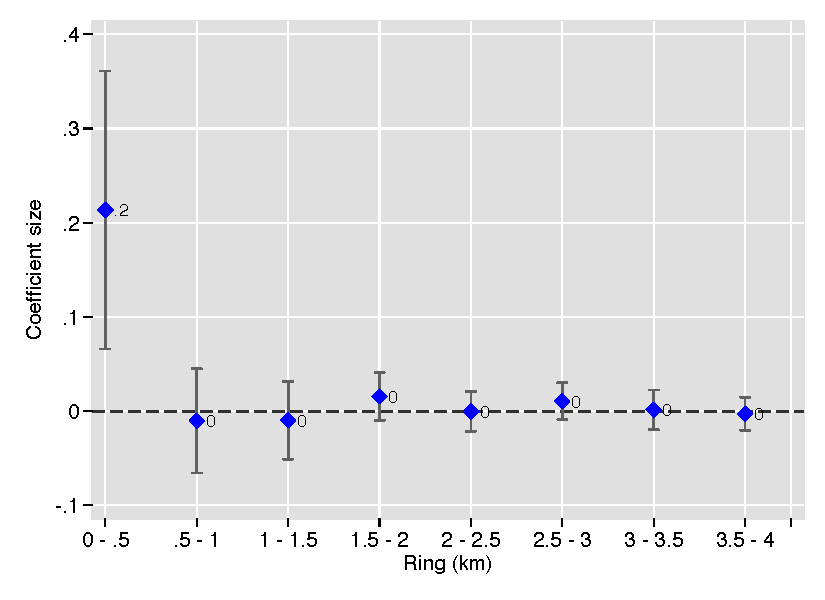
\includegraphics[width=\textwidth,trim={.2cm .2cm .2cm 0cm}, clip=true]{figures/gr_pop.pdf}
        \label{fig:gr_pop}
    \end{subfigure}
    \hfill
    \begin{subfigure}[b]{.49\textwidth}  
        \centering 
        \caption[]{ \small  Houses: Hectares of Overlap }
        \vspace{-1mm}
        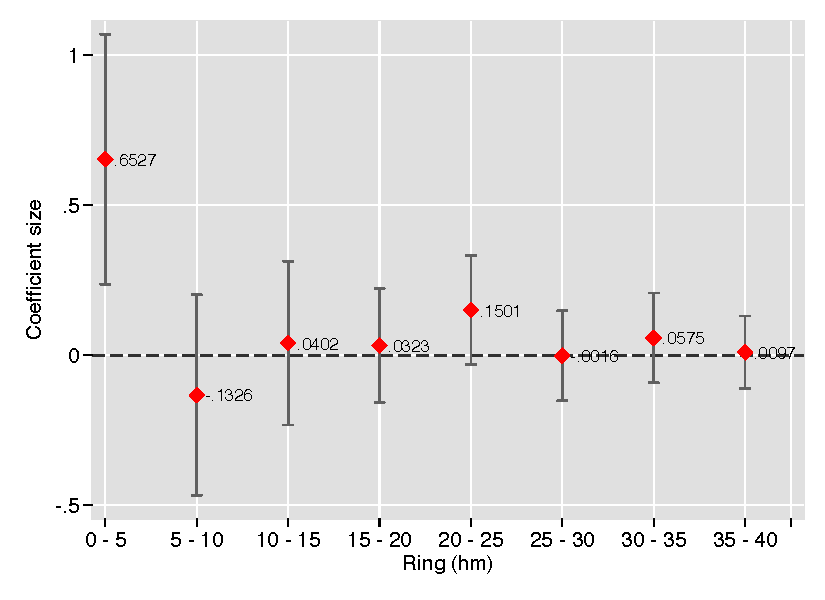
\includegraphics[width=\textwidth,trim={.2cm .2cm .2cm 0cm}, clip=true]{figures/gr_house.pdf}
        \label{fig:gr_house}
    \end{subfigure}
        \vspace{2mm}
    \label{fig:gr_coef_sd}
    \begin{subfigure}[b]{.49\textwidth}
        \centering
        \caption[]{\small People: Sd. Dev. of Hectares of Overlap}  
        \vspace{-1mm}
        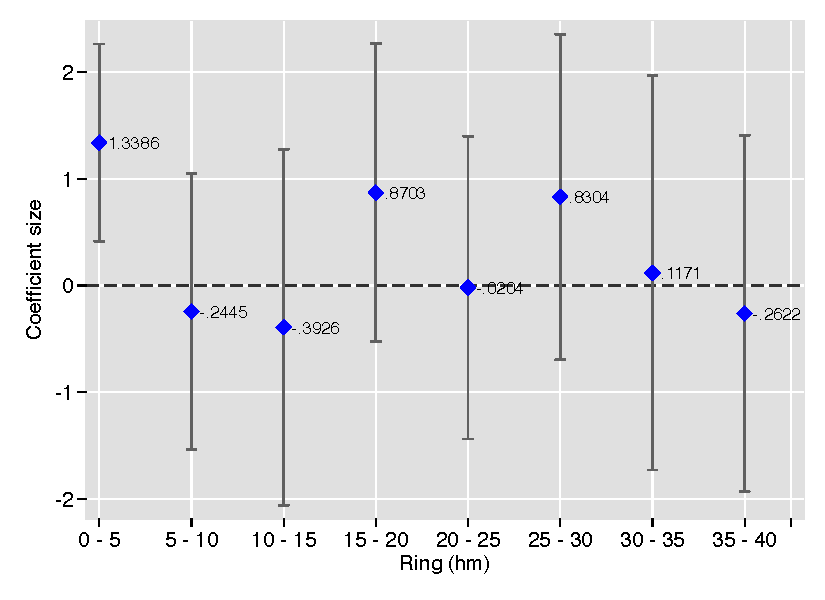
\includegraphics[width=\textwidth,trim={.2cm .2cm .2cm 0cm}, clip=true]{figures/gr_pop_sd.pdf}
        \label{fig:gr_pop_sd}
    \end{subfigure}
    \hfill
    \begin{subfigure}[b]{.49\textwidth}  
        \centering 
        \caption[]{\small Houses: Sd. Dev. of Hectares of Overlap}
        \vspace{-1mm}
        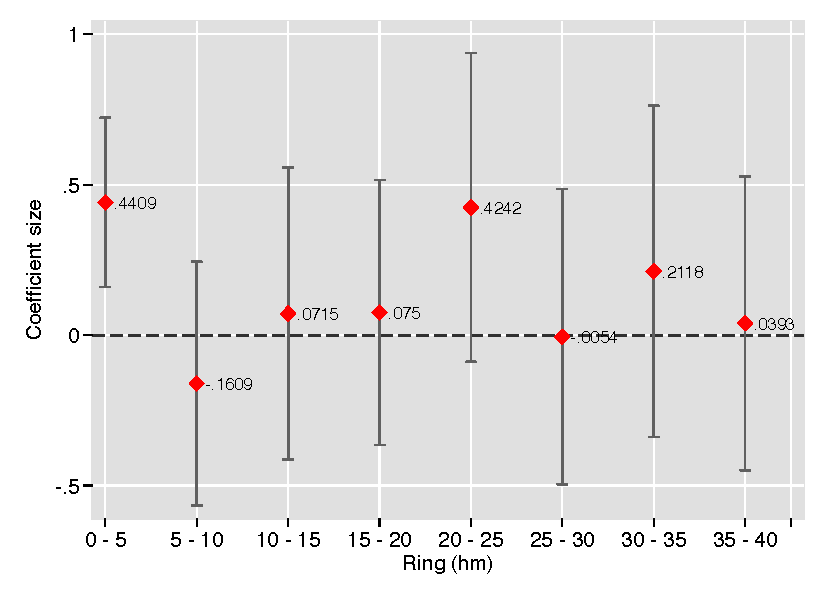
\includegraphics[width=\textwidth,trim={.2cm .2cm .2cm 0cm}, clip=true]{figures/gr_house_sd.pdf}
        \label{fig:gr_house_sd}
    \end{subfigure}
{\footnotesize Figures \ref{fig:gr_pop} and \ref{fig:gr_house} compute overlap in terms of hectares.  Figures \ref{fig:gr_pop_sd} and \ref{fig:gr_house_sd} normalize hectares of overlap by their standard deviations to account for how further rings have larger areas by construction (as shown in Table~\ref{table:spatialsummary}).  Confidence intervals are at the 95\% level. }
\end{figure*} 


{
\scriptsize
\begin{longtable}{lCCCCC}
\caption{Full Estimates: Population and Housing}\label{table:main_full}\\
\toprule
                    &(1)&(2)&(3)&(4)&(5)\\[.5em] &People                   &      Houses                   &Formal Houses                   &Informal Houses                   &Informal Backyard Houses \\ \midrule \\[-.6em]                   \\
Constructed $\times$ Post $\times$ \\[.5em]  \hspace{2.5em} \hspace{1.5em}Plot footprint&      25.737\textsuperscript{a}&       9.102\textsuperscript{a}&       6.629\textsuperscript{a}&       2.473\textsuperscript{b}&       6.648\textsuperscript{a}\\
                    &     (4.630)                   &     (1.544)                   &     (0.812)                   &     (1.044)                   &     (1.157)                   \\[.01em]
\hspace{2em}  Ring Overlap with Project :    \\[.5em]\hspace{2.5em} 0-5  &       0.213\textsuperscript{a}&       0.070\textsuperscript{a}&       0.023\textsuperscript{b}&       0.047\textsuperscript{b}&       0.037\textsuperscript{a}\\
                    &     (0.075)                   &     (0.023)                   &     (0.011)                   &     (0.019)                   &     (0.013)                   \\[0.001em]
\hspace{2.5em} 5-10 &      -0.010                   &      -0.007                   &       0.003                   &      -0.010                   &       0.000                   \\
                    &     (0.028)                   &     (0.009)                   &     (0.005)                   &     (0.007)                   &     (0.006)                   \\[0.001em]
\hspace{2.5em} 10-15&      -0.010                   &       0.002                   &      -0.004\textsuperscript{c}&       0.006                   &       0.002                   \\
                    &     (0.021)                   &     (0.006)                   &     (0.002)                   &     (0.005)                   &     (0.004)                   \\[0.001em]
\hspace{2.5em} 15-20&       0.016                   &       0.001                   &       0.001                   &       0.000                   &       0.002                   \\
                    &     (0.013)                   &     (0.004)                   &     (0.002)                   &     (0.003)                   &     (0.003)                   \\[0.001em]
\hspace{2.5em} 20-25&      -0.000                   &       0.006                   &       0.002                   &       0.004                   &       0.004                   \\
                    &     (0.011)                   &     (0.004)                   &     (0.002)                   &     (0.003)                   &     (0.003)                   \\[0.001em]
\hspace{2.5em} 25-30&       0.011                   &      -0.000                   &      -0.000                   &       0.000                   &       0.001                   \\
                    &     (0.010)                   &     (0.003)                   &     (0.001)                   &     (0.003)                   &     (0.002)                   \\[0.001em]
\hspace{2.5em} 30-35&       0.001                   &       0.002                   &      -0.000                   &       0.003                   &       0.001                   \\
                    &     (0.011)                   &     (0.003)                   &     (0.001)                   &     (0.003)                   &     (0.002)                   \\[0.001em]
\hspace{2.5em} 35-40&      -0.003                   &       0.000                   &      -0.001                   &       0.001                   &       0.001                   \\
                    &     (0.009)                   &     (0.003)                   &     (0.001)                   &     (0.002)                   &     (0.002)                   \\[0.01em]
Post $\times$ \\[.5em]  \hspace{2.5em} \hspace{1.5em}Plot footprint&       5.243\textsuperscript{c}&       2.692\textsuperscript{a}&       0.924\textsuperscript{a}&       1.768\textsuperscript{a}&       0.514                   \\
                    &     (2.857)                   &     (0.811)                   &     (0.262)                   &     (0.631)                   &     (0.312)                   \\[.01em]
\hspace{2em}  Ring Overlap with Project :    \\[.5em]\hspace{2.5em} 0-5  &      -0.015                   &      -0.010                   &      -0.008                   &      -0.002                   &      -0.013\textsuperscript{c}\\
                    &     (0.049)                   &     (0.015)                   &     (0.007)                   &     (0.012)                   &     (0.007)                   \\[0.001em]
\hspace{2.5em} 5-10 &       0.025                   &       0.015\textsuperscript{b}&       0.006\textsuperscript{b}&       0.009\textsuperscript{c}&       0.006                   \\
                    &     (0.020)                   &     (0.006)                   &     (0.003)                   &     (0.005)                   &     (0.004)                   \\[0.001em]
\hspace{2.5em} 10-15&       0.007                   &      -0.003                   &       0.002                   &      -0.005                   &      -0.002                   \\
                    &     (0.015)                   &     (0.004)                   &     (0.002)                   &     (0.004)                   &     (0.003)                   \\[0.001em]
\hspace{2.5em} 15-20&       0.007                   &       0.003                   &      -0.000                   &       0.003                   &       0.003                   \\
                    &     (0.010)                   &     (0.003)                   &     (0.002)                   &     (0.002)                   &     (0.002)                   \\[0.001em]
\hspace{2.5em} 20-25&       0.004                   &       0.000                   &      -0.001                   &       0.001                   &       0.002                   \\
                    &     (0.009)                   &     (0.003)                   &     (0.001)                   &     (0.002)                   &     (0.002)                   \\[0.001em]
\hspace{2.5em} 25-30&      -0.002                   &       0.002                   &       0.000                   &       0.001                   &       0.000                   \\
                    &     (0.007)                   &     (0.002)                   &     (0.001)                   &     (0.002)                   &     (0.001)                   \\[0.001em]
\hspace{2.5em} 30-35&      -0.003                   &      -0.002                   &       0.001                   &      -0.003\textsuperscript{c}&      -0.002                   \\
                    &     (0.008)                   &     (0.002)                   &     (0.001)                   &     (0.002)                   &     (0.001)                   \\[0.001em]
\hspace{2.5em} 35-40&      -0.001                   &       0.002                   &       0.001                   &       0.001                   &       0.001                   \\
                    &     (0.007)                   &     (0.002)                   &     (0.001)                   &     (0.002)                   &     (0.002)                   \\[0.01em]
Constructed $\times$ \\[.5em]  \hspace{2.5em} \hspace{1.5em}Plot footprint&      26.324\textsuperscript{a}&       8.830\textsuperscript{a}&       1.855\textsuperscript{a}&       6.975\textsuperscript{a}&       0.615\textsuperscript{b}\\
                    &     (5.841)                   &     (1.820)                   &     (0.572)                   &     (1.565)                   &     (0.296)                   \\[.01em]
\hspace{2em}  Ring Overlap with Project :    \\[.5em]\hspace{2.5em} 0-5  &       0.095                   &       0.015                   &       0.005                   &       0.010                   &       0.002                   \\
                    &     (0.084)                   &     (0.031)                   &     (0.016)                   &     (0.021)                   &     (0.011)                   \\[0.001em]
\hspace{2.5em} 5-10 &       0.064\textsuperscript{c}&       0.023\textsuperscript{c}&       0.011                   &       0.012                   &       0.009\textsuperscript{c}\\
                    &     (0.039)                   &     (0.013)                   &     (0.007)                   &     (0.009)                   &     (0.005)                   \\[0.001em]
\hspace{2.5em} 10-15&       0.046\textsuperscript{c}&       0.018\textsuperscript{b}&       0.010\textsuperscript{c}&       0.009\textsuperscript{c}&       0.006                   \\
                    &     (0.028)                   &     (0.009)                   &     (0.006)                   &     (0.005)                   &     (0.003)                   \\[0.001em]
\hspace{2.5em} 15-20&       0.043                   &       0.009                   &       0.005                   &       0.004                   &       0.003                   \\
                    &     (0.027)                   &     (0.008)                   &     (0.004)                   &     (0.005)                   &     (0.003)                   \\[0.001em]
\hspace{2.5em} 20-25&       0.017                   &       0.005                   &       0.002                   &       0.004                   &       0.000                   \\
                    &     (0.017)                   &     (0.005)                   &     (0.003)                   &     (0.003)                   &     (0.002)                   \\[0.001em]
\hspace{2.5em} 25-30&      -0.016                   &      -0.004                   &      -0.000                   &      -0.004                   &      -0.001                   \\
                    &     (0.018)                   &     (0.004)                   &     (0.003)                   &     (0.003)                   &     (0.002)                   \\[0.001em]
\hspace{2.5em} 30-35&       0.026                   &       0.010\textsuperscript{b}&       0.004                   &       0.006\textsuperscript{b}&       0.004\textsuperscript{b}\\
                    &     (0.021)                   &     (0.005)                   &     (0.003)                   &     (0.003)                   &     (0.002)                   \\[0.001em]
\hspace{2.5em} 35-40&      -0.000                   &       0.001                   &       0.001                   &       0.000                   &       0.001                   \\
                    &     (0.020)                   &     (0.005)                   &     (0.003)                   &     (0.002)                   &     (0.002)                   \\[0.01em]
Plot footprint      &       0.507                   &       1.225                   &      -0.497                   &       1.722\textsuperscript{a}&       0.033                   \\
                    &     (2.936)                   &     (0.868)                   &     (0.389)                   &     (0.640)                   &     (0.138)                   \\[.01em]
 Ring Overlap with Project :    \\[.5em]\hspace{2.5em} 0-5  &      -0.002                   &       0.004                   &      -0.010                   &       0.013                   &      -0.006                   \\
                    &     (0.045)                   &     (0.016)                   &     (0.010)                   &     (0.010)                   &     (0.005)                   \\[0.001em]
\hspace{2.5em} 5-10 &      -0.004                   &       0.005                   &      -0.000                   &       0.005                   &      -0.003                   \\
                    &     (0.022)                   &     (0.008)                   &     (0.004)                   &     (0.005)                   &     (0.002)                   \\[0.001em]
\hspace{2.5em} 10-15&      -0.029\textsuperscript{c}&      -0.010\textsuperscript{c}&      -0.002                   &      -0.008\textsuperscript{b}&      -0.004\textsuperscript{a}\\
                    &     (0.017)                   &     (0.005)                   &     (0.004)                   &     (0.003)                   &     (0.001)                   \\[0.001em]
\hspace{2.5em} 15-20&       0.011                   &       0.006                   &       0.003                   &       0.004                   &       0.002                   \\
                    &     (0.017)                   &     (0.005)                   &     (0.003)                   &     (0.003)                   &     (0.002)                   \\[0.001em]
\hspace{2.5em} 20-25&      -0.001                   &       0.001                   &       0.002                   &      -0.001                   &       0.001                   \\
                    &     (0.011)                   &     (0.003)                   &     (0.002)                   &     (0.002)                   &     (0.001)                   \\[0.001em]
\hspace{2.5em} 25-30&       0.008                   &       0.001                   &       0.000                   &       0.001                   &       0.000                   \\
                    &     (0.012)                   &     (0.003)                   &     (0.002)                   &     (0.002)                   &     (0.001)                   \\[0.001em]
\hspace{2.5em} 30-35&      -0.005                   &      -0.003                   &      -0.001                   &      -0.001                   &      -0.001                   \\
                    &     (0.018)                   &     (0.004)                   &     (0.002)                   &     (0.002)                   &     (0.001)                   \\[0.001em]
\hspace{2.5em} 35-40&       0.010                   &       0.004                   &       0.001                   &       0.002                   &       0.002                   \\
                    &     (0.015)                   &     (0.004)                   &     (0.002)                   &     (0.002)                   &     (0.001)                   \\[0.01em]
Post                &       3.326\textsuperscript{a}&       0.421\textsuperscript{a}&       0.040                   &       0.382\textsuperscript{a}&       0.271\textsuperscript{a}\\
                    &     (0.643)                   &     (0.132)                   &     (0.040)                   &     (0.111)                   &     (0.101)                   \\[.5em]
Mean Pre            &      13.420                   &       3.167                   &       1.798                   &       1.370                   &       0.521                   \\
Mean Post           &      19.272                   &       4.813                   &       2.417                   &       2.396                   &       1.521                   \\
R$^2$               &       0.090                   &       0.113                   &       0.081                   &       0.093                   &       0.079                   \\
N                   &     701,395                   &     871,778                   &     871,778                   &     871,778                   &     871,778                   \\

\bottomrule
\end{longtable}
}






% {
% \scriptsize
% \begin{longtable}{lCCCCC}
% \caption{Full Estimates: Public Services}\label{table:inf_census_full}\\
% \toprule
%                     &(1)&(2)&(3)&(4)&(5)\\[.5em] &Total Rooms                   &   Own House                   &Electric Lighting                   &Flush Toilet                   &Piped Water Inside\\ \midrule \\[-.6em]                   \\
Constructed $\times$ Post $\times$ \\[.5em]  \hspace{2.5em} \hspace{1.5em}Plot footprint&        0.35                   &        0.04                   &        0.12\textsuperscript{b}&        0.24\textsuperscript{a}&        0.28\textsuperscript{a}\\
                    &      (0.29)                   &      (0.05)                   &      (0.06)                   &      (0.06)                   &      (0.05)                   \\[.3em]
\hspace{2em} \% Buffer Overlap with Project :    \\[1em]\hspace{2.5em} 0-.5 &        0.43                   &        0.06                   &        0.04                   &        0.08                   &        0.01                   \\
                    &      (0.28)                   &      (0.07)                   &      (0.09)                   &      (0.07)                   &      (0.07)                   \\[0.3em]
\hspace{2.5em} .5-1 &       -0.14                   &       -0.19\textsuperscript{b}&       -0.06                   &       -0.04                   &        0.18\textsuperscript{b}\\
                    &      (0.35)                   &      (0.10)                   &      (0.11)                   &      (0.09)                   &      (0.09)                   \\[0.3em]
\hspace{2.5em} 1-1.5&       -0.04                   &        0.14                   &        0.02                   &        0.14                   &        0.02                   \\
                    &      (0.39)                   &      (0.11)                   &      (0.11)                   &      (0.10)                   &      (0.10)                   \\[0.3em]
\hspace{2.5em} 1.5-2&       -0.47                   &       -0.06                   &        0.08                   &        0.14                   &        0.24\textsuperscript{b}\\
                    &      (0.47)                   &      (0.10)                   &      (0.11)                   &      (0.10)                   &      (0.11)                   \\[0.3em]
\hspace{2.5em} 2-2.5&        0.85                   &        0.22\textsuperscript{c}&        0.04                   &       -0.09                   &       -0.04                   \\
                    &      (0.62)                   &      (0.12)                   &      (0.12)                   &      (0.11)                   &      (0.12)                   \\[0.3em]
\hspace{2.5em} 2.5-3&       -1.19                   &       -0.08                   &        0.14                   &        0.14                   &        0.22                   \\
                    &      (0.75)                   &      (0.12)                   &      (0.14)                   &      (0.12)                   &      (0.13)                   \\[0.3em]
\hspace{2.5em} 3-3.5&        0.57                   &       -0.04                   &       -0.00                   &       -0.01                   &       -0.15                   \\
                    &      (0.88)                   &      (0.15)                   &      (0.17)                   &      (0.15)                   &      (0.20)                   \\[0.3em]
\hspace{2.5em} 3.5-4&       -2.41\textsuperscript{c}&        0.01                   &       -0.30                   &        0.04                   &        0.54\textsuperscript{b}\\
                    &      (1.36)                   &      (0.22)                   &      (0.30)                   &      (0.27)                   &      (0.23)                   \\[0.9em]
Post $\times$ \\[.5em]  \hspace{2.5em} \hspace{1.5em}Plot footprint&       -0.16                   &        0.02                   &        0.06                   &        0.01                   &       -0.12\textsuperscript{a}\\
                    &      (0.26)                   &      (0.04)                   &      (0.04)                   &      (0.04)                   &      (0.04)                   \\[.3em]
\hspace{2em} \% Buffer Overlap with Project :    \\[1em]\hspace{2.5em} 0-.5 &       -0.49\textsuperscript{b}&       -0.05                   &       -0.10\textsuperscript{c}&       -0.09\textsuperscript{c}&       -0.10\textsuperscript{b}\\
                    &      (0.21)                   &      (0.04)                   &      (0.06)                   &      (0.05)                   &      (0.05)                   \\[0.3em]
\hspace{2.5em} .5-1 &       -0.15                   &        0.07                   &        0.10                   &        0.08                   &       -0.05                   \\
                    &      (0.29)                   &      (0.07)                   &      (0.09)                   &      (0.06)                   &      (0.06)                   \\[0.3em]
\hspace{2.5em} 1-1.5&        0.09                   &       -0.06                   &       -0.00                   &       -0.02                   &       -0.05                   \\
                    &      (0.32)                   &      (0.08)                   &      (0.08)                   &      (0.06)                   &      (0.07)                   \\[0.3em]
\hspace{2.5em} 1.5-2&        0.16                   &        0.02                   &       -0.07                   &       -0.13\textsuperscript{c}&       -0.11                   \\
                    &      (0.37)                   &      (0.08)                   &      (0.09)                   &      (0.07)                   &      (0.08)                   \\[0.3em]
\hspace{2.5em} 2-2.5&       -0.19                   &       -0.12                   &        0.06                   &        0.13\textsuperscript{c}&        0.01                   \\
                    &      (0.44)                   &      (0.09)                   &      (0.08)                   &      (0.08)                   &      (0.09)                   \\[0.3em]
\hspace{2.5em} 2.5-3&        0.64                   &        0.07                   &        0.01                   &       -0.08                   &       -0.13                   \\
                    &      (0.57)                   &      (0.10)                   &      (0.10)                   &      (0.09)                   &      (0.09)                   \\[0.3em]
\hspace{2.5em} 3-3.5&       -0.27                   &        0.10                   &       -0.06                   &        0.05                   &        0.17                   \\
                    &      (0.66)                   &      (0.11)                   &      (0.13)                   &      (0.13)                   &      (0.17)                   \\[0.3em]
\hspace{2.5em} 3.5-4&        2.16\textsuperscript{b}&       -0.04                   &        0.42\textsuperscript{c}&        0.02                   &       -0.34\textsuperscript{c}\\
                    &      (1.09)                   &      (0.16)                   &      (0.22)                   &      (0.19)                   &      (0.19)                   \\[0.9em]
Constructed $\times$ \\[.5em]  \hspace{2.5em} \hspace{1.5em}Plot footprint&       -0.26                   &        0.07                   &        0.01                   &        0.06                   &       -0.13\textsuperscript{b}\\
                    &      (0.33)                   &      (0.06)                   &      (0.10)                   &      (0.10)                   &      (0.06)                   \\[.3em]
\hspace{2em} \% Buffer Overlap with Project :    \\[1em]\hspace{2.5em} 0-.5 &       -1.20\textsuperscript{a}&       -0.12                   &       -0.12                   &       -0.12                   &       -0.16\textsuperscript{b}\\
                    &      (0.31)                   &      (0.07)                   &      (0.08)                   &      (0.07)                   &      (0.07)                   \\[0.3em]
\hspace{2.5em} .5-1 &        0.03                   &        0.10                   &        0.05                   &        0.07                   &       -0.19\textsuperscript{b}\\
                    &      (0.37)                   &      (0.09)                   &      (0.08)                   &      (0.09)                   &      (0.09)                   \\[0.3em]
\hspace{2.5em} 1-1.5&        0.26                   &        0.13                   &       -0.01                   &       -0.08                   &        0.05                   \\
                    &      (0.46)                   &      (0.12)                   &      (0.11)                   &      (0.11)                   &      (0.12)                   \\[0.3em]
\hspace{2.5em} 1.5-2&       -0.29                   &        0.04                   &        0.12                   &        0.15                   &       -0.05                   \\
                    &      (0.53)                   &      (0.11)                   &      (0.12)                   &      (0.12)                   &      (0.12)                   \\[0.3em]
\hspace{2.5em} 2-2.5&       -0.24                   &        0.00                   &       -0.02                   &        0.07                   &        0.12                   \\
                    &      (0.53)                   &      (0.13)                   &      (0.13)                   &      (0.13)                   &      (0.14)                   \\[0.3em]
\hspace{2.5em} 2.5-3&        0.26                   &        0.10                   &       -0.04                   &        0.01                   &       -0.11                   \\
                    &      (0.60)                   &      (0.13)                   &      (0.16)                   &      (0.17)                   &      (0.15)                   \\[0.3em]
\hspace{2.5em} 3-3.5&       -0.59                   &       -0.00                   &       -0.03                   &       -0.05                   &       -0.02                   \\
                    &      (0.82)                   &      (0.17)                   &      (0.19)                   &      (0.19)                   &      (0.18)                   \\[0.3em]
\hspace{2.5em} 3.5-4&        0.95                   &        0.00                   &        0.10                   &        0.13                   &       -0.24                   \\
                    &      (1.17)                   &      (0.32)                   &      (0.36)                   &      (0.39)                   &      (0.32)                   \\[0.9em]
\hspace{2.5em} \hspace{1.5em}Plot footprint&       -0.79\textsuperscript{b}&       -0.11\textsuperscript{c}&       -0.25\textsuperscript{b}&       -0.22\textsuperscript{b}&       -0.16\textsuperscript{a}\\
                    &      (0.33)                   &      (0.06)                   &      (0.10)                   &      (0.10)                   &      (0.06)                   \\[.3em]
\hspace{2.5em} 0-.5 &        0.23                   &        0.05                   &        0.02                   &        0.04                   &        0.06                   \\
                    &      (0.23)                   &      (0.05)                   &      (0.05)                   &      (0.05)                   &      (0.05)                   \\[0.3em]
\hspace{2.5em} .5-1 &        0.03                   &        0.03                   &       -0.08                   &       -0.10                   &        0.01                   \\
                    &      (0.27)                   &      (0.07)                   &      (0.06)                   &      (0.07)                   &      (0.06)                   \\[0.3em]
\hspace{2.5em} 1-1.5&       -0.31                   &       -0.06                   &        0.00                   &        0.07                   &        0.08                   \\
                    &      (0.36)                   &      (0.09)                   &      (0.08)                   &      (0.08)                   &      (0.09)                   \\[0.3em]
\hspace{2.5em} 1.5-2&        0.22                   &        0.04                   &       -0.06                   &       -0.00                   &       -0.04                   \\
                    &      (0.42)                   &      (0.08)                   &      (0.09)                   &      (0.09)                   &      (0.09)                   \\[0.3em]
\hspace{2.5em} 2-2.5&       -0.13                   &       -0.03                   &       -0.04                   &       -0.13                   &       -0.12                   \\
                    &      (0.41)                   &      (0.09)                   &      (0.09)                   &      (0.09)                   &      (0.10)                   \\[0.3em]
\hspace{2.5em} 2.5-3&       -0.52                   &       -0.07                   &       -0.08                   &       -0.04                   &       -0.03                   \\
                    &      (0.46)                   &      (0.10)                   &      (0.12)                   &      (0.13)                   &      (0.12)                   \\[0.3em]
\hspace{2.5em} 3-3.5&        0.75                   &        0.04                   &        0.21                   &        0.15                   &        0.05                   \\
                    &      (0.67)                   &      (0.13)                   &      (0.14)                   &      (0.15)                   &      (0.13)                   \\[0.3em]
\hspace{2.5em} 3.5-4&       -2.22\textsuperscript{b}&       -0.09                   &       -0.55\textsuperscript{b}&       -0.36                   &       -0.20                   \\
                    &      (1.02)                   &      (0.22)                   &      (0.27)                   &      (0.33)                   &      (0.26)                   \\[0.9em]
\textsc{Post}       &        0.41\textsuperscript{a}&       -0.00                   &        0.04\textsuperscript{b}&        0.03                   &        0.17\textsuperscript{a}\\
                    &      (0.08)                   &      (0.01)                   &      (0.02)                   &      (0.02)                   &      (0.02)                   \\[.5em]
Mean Pre            &        3.50                   &        0.35                   &        0.69                   &        0.70                   &        0.41                   \\
Mean Post           &        3.98                   &        0.35                   &        0.77                   &        0.75                   &        0.58                   \\
R$^2$               &       0.063                   &       0.010                   &       0.049                   &       0.034                   &       0.102                   \\
N                   &     698,762                   &     699,801                   &     701,296                   &     701,296                   &     701,296                   \\

% \bottomrule
% \end{longtable}
% }


% {
% \scriptsize
% \begin{longtable}{lCCCCC}
% \caption{Full Estimates: Public Service Buildings}\label{table:inf_bblu_full}\\
% \toprule
%                     &(1)&(2)&(3)&(4)\\[.5em] &Water Utility Buildings per $\text{km}^{2}$                    &Electricity Utility Buildings per $\text{km}^{2}$                    &Health Centers per $\text{km}^{2}$                    &Schools per $\text{km}^{2}$ \\ \midrule \\[-.6em]                   \\
Constructed $\times$ Post $\times$ \\[.5em]  \hspace{2.5em} \hspace{1.5em}Plot footprint&       2.454\textsuperscript{a}&       0.062                   &       0.109\textsuperscript{b}&       6.252\textsuperscript{a}\\
                    &     (0.532)                   &     (0.052)                   &     (0.048)                   &     (1.455)                   \\[.3em]
\hspace{2em} \% Buffer Overlap with Project :    \\[1em]\hspace{2.5em} 0-.5 &       0.447                   &       0.813                   &      -2.720                   &      11.696\textsuperscript{c}\\
                    &     (2.251)                   &     (0.546)                   &     (1.781)                   &     (6.951)                   \\[0.3em]
\hspace{2.5em} .5-1 &      -1.155                   &      -0.757                   &       1.790                   &       0.718                   \\
                    &     (2.169)                   &     (0.617)                   &     (1.143)                   &     (6.635)                   \\[0.3em]
\hspace{2.5em} 1-1.5&       1.783                   &       0.039                   &      -1.261                   &       5.767                   \\
                    &     (2.276)                   &     (0.628)                   &     (1.406)                   &     (6.692)                   \\[0.3em]
\hspace{2.5em} 1.5-2&      -1.210                   &      -0.423                   &       1.458                   &      -1.549                   \\
                    &     (2.554)                   &     (0.567)                   &     (1.433)                   &     (6.410)                   \\[0.3em]
\hspace{2.5em} 2-2.5&       8.836\textsuperscript{a}&       0.676                   &      -0.275                   &      -3.149                   \\
                    &     (3.327)                   &     (0.780)                   &     (0.869)                   &     (8.983)                   \\[0.3em]
\hspace{2.5em} 2.5-3&      -4.782                   &      -0.115                   &       0.782                   &      13.426\textsuperscript{c}\\
                    &     (3.076)                   &     (1.037)                   &     (0.754)                   &     (7.623)                   \\[0.3em]
\hspace{2.5em} 3-3.5&      -1.060                   &       0.086                   &      -1.093                   &      -9.997\textsuperscript{c}\\
                    &     (2.633)                   &     (1.032)                   &     (0.975)                   &     (5.986)                   \\[0.3em]
\hspace{2.5em} 3.5-4&       2.717                   &      -0.515                   &       0.805                   &       5.730                   \\
                    &     (1.798)                   &     (0.715)                   &     (0.739)                   &     (4.197)                   \\[0.9em]
Post $\times$ \\[.5em]  \hspace{2.5em} \hspace{1.5em}Plot footprint&       0.381\textsuperscript{b}&      -0.011                   &      -0.021                   &       1.724\textsuperscript{b}\\
                    &     (0.193)                   &     (0.046)                   &     (0.022)                   &     (0.808)                   \\[.3em]
\hspace{2em} \% Buffer Overlap with Project :    \\[1em]\hspace{2.5em} 0-.5 &       0.337                   &       0.055                   &       2.230                   &      -9.866\textsuperscript{a}\\
                    &     (1.357)                   &     (0.369)                   &     (1.607)                   &     (2.922)                   \\[0.3em]
\hspace{2.5em} .5-1 &       0.822                   &       0.084                   &      -1.630\textsuperscript{c}&      11.328\textsuperscript{a}\\
                    &     (1.347)                   &     (0.424)                   &     (0.979)                   &     (4.118)                   \\[0.3em]
\hspace{2.5em} 1-1.5&       1.299                   &       0.633                   &       0.803                   &      -8.767                   \\
                    &     (1.341)                   &     (0.575)                   &     (0.989)                   &     (5.443)                   \\[0.3em]
\hspace{2.5em} 1.5-2&      -1.192                   &      -0.304                   &      -0.370                   &       6.200                   \\
                    &     (1.328)                   &     (0.420)                   &     (0.873)                   &     (6.847)                   \\[0.3em]
\hspace{2.5em} 2-2.5&      -2.205                   &      -0.404                   &      -0.412                   &       5.363                   \\
                    &     (1.708)                   &     (0.476)                   &     (0.524)                   &     (7.265)                   \\[0.3em]
\hspace{2.5em} 2.5-3&       0.999                   &       0.603                   &       0.341                   &     -11.101\textsuperscript{b}\\
                    &     (1.713)                   &     (0.842)                   &     (0.450)                   &     (5.498)                   \\[0.3em]
\hspace{2.5em} 3-3.5&       3.125                   &      -0.203                   &      -0.323                   &      11.732\textsuperscript{a}\\
                    &     (2.136)                   &     (0.833)                   &     (0.751)                   &     (4.473)                   \\[0.3em]
\hspace{2.5em} 3.5-4&      -1.589                   &       0.162                   &       0.240                   &      -5.762\textsuperscript{c}\\
                    &     (1.508)                   &     (0.437)                   &     (0.561)                   &     (3.016)                   \\[0.9em]
Constructed $\times$ \\[.5em]  \hspace{2.5em} \hspace{1.5em}Plot footprint&       1.984\textsuperscript{a}&       0.067                   &       0.106                   &       2.343\textsuperscript{a}\\
                    &     (0.517)                   &     (0.102)                   &     (0.064)                   &     (0.872)                   \\[.3em]
\hspace{2em} \% Buffer Overlap with Project :    \\[1em]\hspace{2.5em} 0-.5 &       0.825                   &      -0.759                   &      -2.023                   &      -7.629                   \\
                    &     (3.105)                   &     (1.114)                   &     (5.623)                   &     (4.804)                   \\[0.3em]
\hspace{2.5em} .5-1 &      -3.522                   &       0.558                   &      -8.895                   &      17.581\textsuperscript{a}\\
                    &     (5.510)                   &     (0.872)                   &     (9.667)                   &     (6.024)                   \\[0.3em]
\hspace{2.5em} 1-1.5&       3.050                   &      -0.239                   &       1.937                   &     -10.770\textsuperscript{c}\\
                    &     (7.308)                   &     (1.138)                   &     (5.042)                   &     (6.507)                   \\[0.3em]
\hspace{2.5em} 1.5-2&       3.178                   &      -0.104                   &       4.414                   &      17.408\textsuperscript{b}\\
                    &     (6.140)                   &     (1.207)                   &     (4.313)                   &     (7.194)                   \\[0.3em]
\hspace{2.5em} 2-2.5&      -1.769                   &       0.572                   &      -5.056                   &     -13.171\textsuperscript{c}\\
                    &     (5.050)                   &     (1.194)                   &     (3.839)                   &     (7.871)                   \\[0.3em]
\hspace{2.5em} 2.5-3&       4.608                   &      -2.835\textsuperscript{b}&       2.093                   &      17.541\textsuperscript{b}\\
                    &     (5.721)                   &     (1.277)                   &     (3.665)                   &     (8.287)                   \\[0.3em]
\hspace{2.5em} 3-3.5&       5.818                   &       3.256\textsuperscript{a}&      -6.545                   &     -13.838\textsuperscript{c}\\
                    &     (6.958)                   &     (1.192)                   &     (7.511)                   &     (8.036)                   \\[0.3em]
\hspace{2.5em} 3.5-4&       0.549                   &      -1.090                   &       7.524                   &      13.632\textsuperscript{c}\\
                    &     (4.619)                   &     (0.945)                   &     (6.329)                   &     (7.093)                   \\[0.9em]
\hspace{2.5em} \hspace{1.5em}Plot footprint&      -0.560\textsuperscript{a}&      -0.329\textsuperscript{a}&      -0.462\textsuperscript{a}&      -0.957                   \\
                    &     (0.139)                   &     (0.092)                   &     (0.106)                   &     (0.630)                   \\[.3em]
\hspace{2.5em} 0-.5 &      -0.576                   &       0.469                   &       4.432                   &      -1.306                   \\
                    &     (2.008)                   &     (0.980)                   &     (5.070)                   &     (2.928)                   \\[0.3em]
\hspace{2.5em} .5-1 &       0.043                   &      -0.368                   &       4.416                   &      -3.467                   \\
                    &     (4.853)                   &     (0.615)                   &     (9.693)                   &     (3.580)                   \\[0.3em]
\hspace{2.5em} 1-1.5&       2.458                   &       0.391                   &       1.616                   &       0.311                   \\
                    &     (5.496)                   &     (0.703)                   &     (4.486)                   &     (4.693)                   \\[0.3em]
\hspace{2.5em} 1.5-2&      -4.253                   &      -0.033                   &      -4.043                   &       1.754                   \\
                    &     (3.744)                   &     (0.773)                   &     (3.550)                   &     (5.441)                   \\[0.3em]
\hspace{2.5em} 2-2.5&       0.809                   &       0.012                   &       2.660                   &       6.801                   \\
                    &     (3.186)                   &     (0.813)                   &     (3.704)                   &     (5.971)                   \\[0.3em]
\hspace{2.5em} 2.5-3&       4.004                   &       1.221                   &      -0.880                   &      -9.877\textsuperscript{c}\\
                    &     (3.246)                   &     (1.125)                   &     (3.726)                   &     (5.646)                   \\[0.3em]
\hspace{2.5em} 3-3.5&      -5.301                   &      -2.608\textsuperscript{b}&       2.173                   &      13.666\textsuperscript{b}\\
                    &     (3.679)                   &     (1.132)                   &     (3.286)                   &     (5.898)                   \\[0.3em]
\hspace{2.5em} 3.5-4&      -0.358                   &       0.606                   &      -3.207                   &      -8.499\textsuperscript{c}\\
                    &     (2.493)                   &     (0.744)                   &     (3.112)                   &     (4.854)                   \\[0.9em]
\textsc{Post}       &       0.150\textsuperscript{b}&       0.083\textsuperscript{a}&       0.047\textsuperscript{a}&       0.362\textsuperscript{a}\\
                    &     (0.059)                   &     (0.017)                   &     (0.015)                   &     (0.136)                   \\[.5em]
Mean Pre            &       1.068                   &       0.384                   &       0.525                   &       2.824                   \\
Mean Post           &       1.602                   &       0.481                   &       0.595                   &       4.212                   \\
R$^2$               &       0.002                   &       0.000                   &       0.001                   &       0.003                   \\
N                   &     871,772                   &     871,772                   &     871,772                   &     871,772                   \\

% \bottomrule
% \end{longtable}
% }


% {
% \scriptsize
% \begin{longtable}{lCCCCC}
% \caption{Full Estimates: Agglomeration Outcomes}\label{table:inf_bblu_full}\\
% \toprule
%                     &(1)&(2)&(3)&(4)\\[.5em] &Businesses per $\text{km}^{2}$                   &Informal Businesses per $\text{km}^{2}$                   &Household Employment                   &Log Household Income\\ \midrule \\[-.6em]                   \\
Constructed $\times$ Post $\times$ \\[.5em]  \hspace{2.5em} \hspace{1.5em}Plot footprint&       5.334\textsuperscript{a}&       3.445\textsuperscript{a}&       0.030                   &       0.019                   \\
                    &     (1.263)                   &     (0.831)                   &     (0.035)                   &     (0.173)                   \\[.3em]
\hspace{2em} \% Buffer Overlap with Project :    \\[1em]\hspace{2.5em} 0-.5 &       4.163                   &       4.250                   &       0.020                   &      -0.080                   \\
                    &     (3.881)                   &     (2.838)                   &     (0.043)                   &     (0.151)                   \\[0.3em]
\hspace{2.5em} .5-1 &       1.466                   &       0.631                   &       0.018                   &      -0.160                   \\
                    &     (3.462)                   &     (2.401)                   &     (0.050)                   &     (0.195)                   \\[0.3em]
\hspace{2.5em} 1-1.5&       3.833                   &      -0.148                   &       0.052                   &      -0.211                   \\
                    &     (5.116)                   &     (3.333)                   &     (0.061)                   &     (0.214)                   \\[0.3em]
\hspace{2.5em} 1.5-2&      -2.156                   &       1.970                   &       0.016                   &      -0.207                   \\
                    &     (6.966)                   &     (4.753)                   &     (0.064)                   &     (0.211)                   \\[0.3em]
\hspace{2.5em} 2-2.5&      -0.647                   &      -2.774                   &       0.036                   &      -0.016                   \\
                    &     (5.907)                   &     (4.699)                   &     (0.071)                   &     (0.228)                   \\[0.3em]
\hspace{2.5em} 2.5-3&      11.699                   &       5.777                   &       0.120\textsuperscript{c}&      -0.208                   \\
                    &     (7.187)                   &     (5.605)                   &     (0.073)                   &     (0.288)                   \\[0.3em]
\hspace{2.5em} 3-3.5&      -1.361                   &      -0.007                   &      -0.031                   &      -0.194                   \\
                    &     (6.549)                   &     (4.994)                   &     (0.084)                   &     (0.370)                   \\[0.3em]
\hspace{2.5em} 3.5-4&      -2.002                   &       1.098                   &       0.145                   &      -0.116                   \\
                    &     (4.607)                   &     (3.418)                   &     (0.128)                   &     (0.536)                   \\[0.9em]
Post $\times$ \\[.5em]  \hspace{2.5em} \hspace{1.5em}Plot footprint&      -0.373                   &       0.140                   &       0.053\textsuperscript{c}&      -0.436\textsuperscript{a}\\
                    &     (0.376)                   &     (0.230)                   &     (0.028)                   &     (0.165)                   \\[.3em]
\hspace{2em} \% Buffer Overlap with Project :    \\[1em]\hspace{2.5em} 0-.5 &       0.630                   &       0.064                   &       0.028                   &      -0.282\textsuperscript{b}\\
                    &     (1.945)                   &     (1.348)                   &     (0.028)                   &     (0.114)                   \\[0.3em]
\hspace{2.5em} .5-1 &      -2.332                   &      -1.539                   &       0.024                   &      -0.097                   \\
                    &     (1.945)                   &     (1.418)                   &     (0.040)                   &     (0.161)                   \\[0.3em]
\hspace{2.5em} 1-1.5&      -3.376                   &      -1.870                   &      -0.011                   &       0.085                   \\
                    &     (3.086)                   &     (2.255)                   &     (0.040)                   &     (0.165)                   \\[0.3em]
\hspace{2.5em} 1.5-2&       8.408                   &       5.605                   &       0.007                   &       0.044                   \\
                    &     (5.336)                   &     (3.757)                   &     (0.053)                   &     (0.167)                   \\[0.3em]
\hspace{2.5em} 2-2.5&      -5.532                   &      -3.398                   &      -0.006                   &      -0.022                   \\
                    &     (4.217)                   &     (3.255)                   &     (0.051)                   &     (0.170)                   \\[0.3em]
\hspace{2.5em} 2.5-3&      -0.384                   &       0.831                   &       0.002                   &      -0.019                   \\
                    &     (4.444)                   &     (3.141)                   &     (0.055)                   &     (0.217)                   \\[0.3em]
\hspace{2.5em} 3-3.5&      -0.600                   &       0.084                   &      -0.030                   &       0.237                   \\
                    &     (4.247)                   &     (2.872)                   &     (0.064)                   &     (0.285)                   \\[0.3em]
\hspace{2.5em} 3.5-4&       1.776                   &      -0.707                   &       0.094                   &      -0.391                   \\
                    &     (2.851)                   &     (2.328)                   &     (0.106)                   &     (0.423)                   \\[0.9em]
Constructed $\times$ \\[.5em]  \hspace{2.5em} \hspace{1.5em}Plot footprint&       0.868                   &       0.466                   &      -0.078                   &      -0.362\textsuperscript{b}\\
                    &     (0.628)                   &     (0.293)                   &     (0.050)                   &     (0.152)                   \\[.3em]
\hspace{2em} \% Buffer Overlap with Project :    \\[1em]\hspace{2.5em} 0-.5 &       3.546                   &      -0.019                   &      -0.096\textsuperscript{b}&      -0.512\textsuperscript{a}\\
                    &     (5.563)                   &     (1.894)                   &     (0.043)                   &     (0.138)                   \\[0.3em]
\hspace{2.5em} .5-1 &       1.461                   &       1.351                   &      -0.049                   &      -0.234                   \\
                    &     (5.886)                   &     (2.549)                   &     (0.052)                   &     (0.153)                   \\[0.3em]
\hspace{2.5em} 1-1.5&       6.583                   &      -2.003                   &      -0.108\textsuperscript{c}&      -0.048                   \\
                    &     (8.324)                   &     (2.178)                   &     (0.059)                   &     (0.198)                   \\[0.3em]
\hspace{2.5em} 1.5-2&      -2.179                   &       1.400                   &      -0.048                   &      -0.205                   \\
                    &     (9.771)                   &     (2.813)                   &     (0.073)                   &     (0.243)                   \\[0.3em]
\hspace{2.5em} 2-2.5&      13.838                   &       5.847\textsuperscript{c}&      -0.079                   &      -0.081                   \\
                    &    (12.109)                   &     (3.510)                   &     (0.070)                   &     (0.244)                   \\[0.3em]
\hspace{2.5em} 2.5-3&     -15.119                   &      -1.268                   &      -0.073                   &      -0.143                   \\
                    &    (12.320)                   &     (3.455)                   &     (0.073)                   &     (0.309)                   \\[0.3em]
\hspace{2.5em} 3-3.5&      10.321                   &      -1.983                   &      -0.055                   &      -0.230                   \\
                    &    (15.877)                   &     (4.183)                   &     (0.093)                   &     (0.453)                   \\[0.3em]
\hspace{2.5em} 3.5-4&     -19.716                   &       3.669                   &       0.031                   &      -0.428                   \\
                    &    (14.119)                   &     (3.086)                   &     (0.140)                   &     (0.839)                   \\[0.9em]
\hspace{2.5em} \hspace{1.5em}Plot footprint&      -6.273\textsuperscript{a}&       0.237                   &      -0.155\textsuperscript{a}&      -0.198                   \\
                    &     (1.539)                   &     (0.223)                   &     (0.044)                   &     (0.163)                   \\[.3em]
\hspace{2.5em} 0-.5 &      -1.546                   &      -0.285                   &      -0.061\textsuperscript{b}&       0.231\textsuperscript{b}\\
                    &     (3.411)                   &     (0.951)                   &     (0.029)                   &     (0.108)                   \\[0.3em]
\hspace{2.5em} .5-1 &      -3.691                   &       0.256                   &      -0.040                   &       0.050                   \\
                    &     (3.220)                   &     (0.998)                   &     (0.037)                   &     (0.109)                   \\[0.3em]
\hspace{2.5em} 1-1.5&      -9.849                   &      -1.000                   &       0.012                   &      -0.026                   \\
                    &     (6.515)                   &     (1.082)                   &     (0.039)                   &     (0.161)                   \\[0.3em]
\hspace{2.5em} 1.5-2&       4.458                   &       1.668                   &      -0.044                   &       0.015                   \\
                    &     (8.394)                   &     (1.566)                   &     (0.054)                   &     (0.207)                   \\[0.3em]
\hspace{2.5em} 2-2.5&      -4.724                   &      -2.720\textsuperscript{b}&       0.023                   &      -0.083                   \\
                    &     (8.715)                   &     (1.264)                   &     (0.052)                   &     (0.197)                   \\[0.3em]
\hspace{2.5em} 2.5-3&       1.582                   &       0.818                   &      -0.071                   &      -0.273                   \\
                    &     (9.509)                   &     (1.970)                   &     (0.055)                   &     (0.257)                   \\[0.3em]
\hspace{2.5em} 3-3.5&       4.490                   &       1.757                   &       0.118\textsuperscript{c}&       0.369                   \\
                    &    (14.756)                   &     (1.783)                   &     (0.066)                   &     (0.322)                   \\[0.3em]
\hspace{2.5em} 3.5-4&      -8.429                   &      -1.535                   &      -0.365\textsuperscript{a}&      -0.613                   \\
                    &    (13.051)                   &     (1.143)                   &     (0.103)                   &     (0.655)                   \\[0.9em]
\textsc{Post}       &       1.232\textsuperscript{a}&       0.236\textsuperscript{a}&       0.021\textsuperscript{a}&       1.187\textsuperscript{a}\\
                    &     (0.178)                   &     (0.085)                   &     (0.007)                   &     (0.045)                   \\[.5em]
Mean Pre            &       5.584                   &       0.237                   &       0.815                   &       7.310                   \\
Mean Post           &       7.351                   &       0.873                   &       0.863                   &       8.406                   \\
R$^2$               &       0.001                   &       0.002                   &       0.149                   &       0.380                   \\
N                   &     871,772                   &     871,772                   &     698,873                   &     699,171                   \\

% \bottomrule
% \end{longtable}
% }










%%%%%%%%%%%% OLD FIGURESSS! !!!! %%%%%%%%%%%%%%%
%%%%%%%%%%%% OLD FIGURESSS! !!!! %%%%%%%%%%%%%%%
%%%%%%%%%%%% OLD FIGURESSS! !!!! %%%%%%%%%%%%%%%
%%%%%%%%%%%% OLD FIGURESSS! !!!! %%%%%%%%%%%%%%%


% \begin{figure}[ht!]
% \caption{Transaction Price Histogram}\label{figure:transactionhist}
% \centering
% 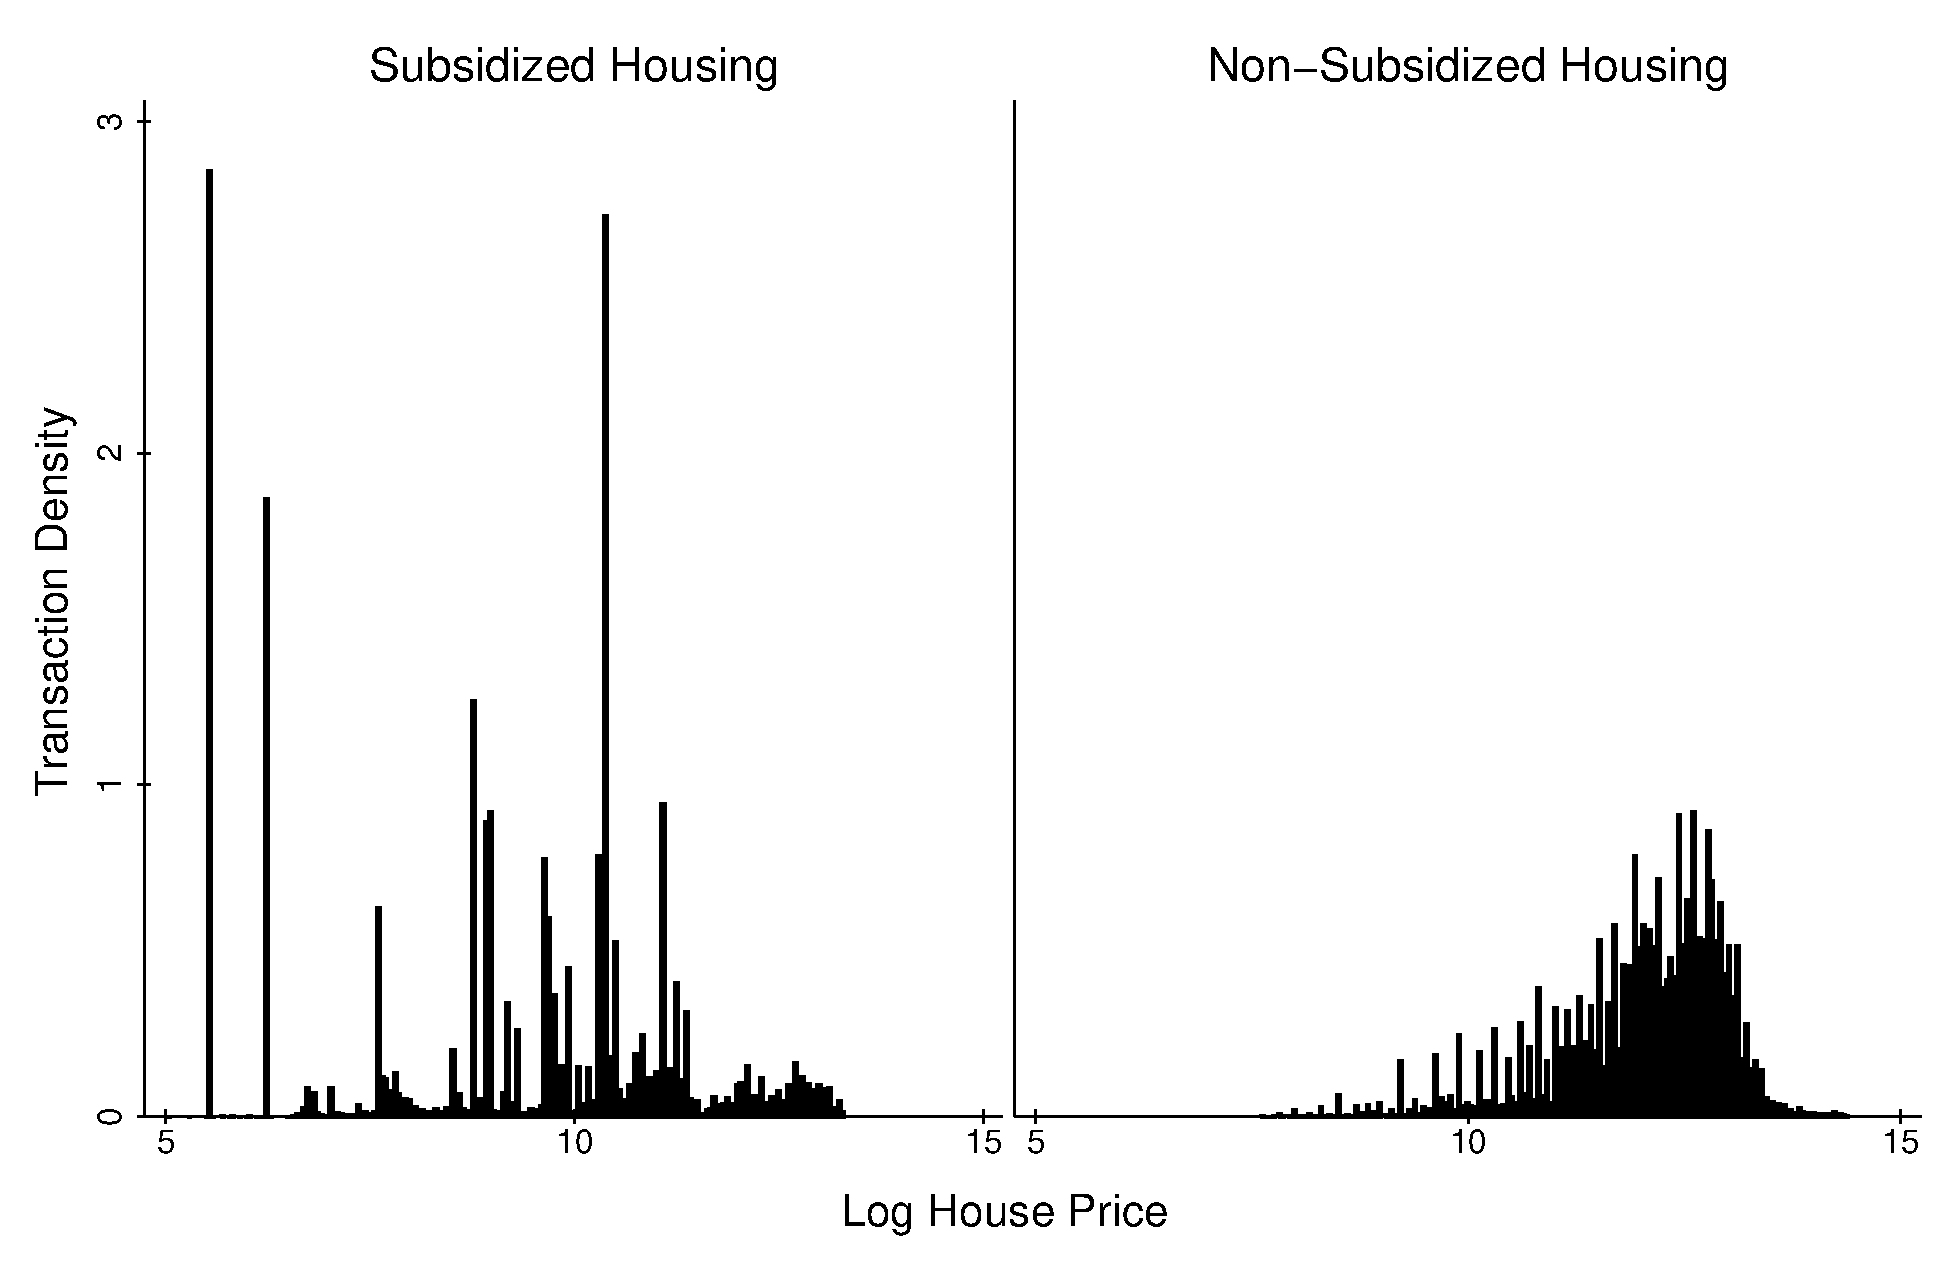
\includegraphics[scale=.4,trim={0cm 0cm -1cm 0cm}]{figures/summary_pricedist.pdf}
% \\
% \footnotesize{Note: Transactions are censored at R100,000.}
% \end{figure}

% \begin{figure}[h!]
% \centering
% \caption{Housing Transactions relative to Each Project's Modal Transaction Month}
% \label{appendix:histfreq}
% 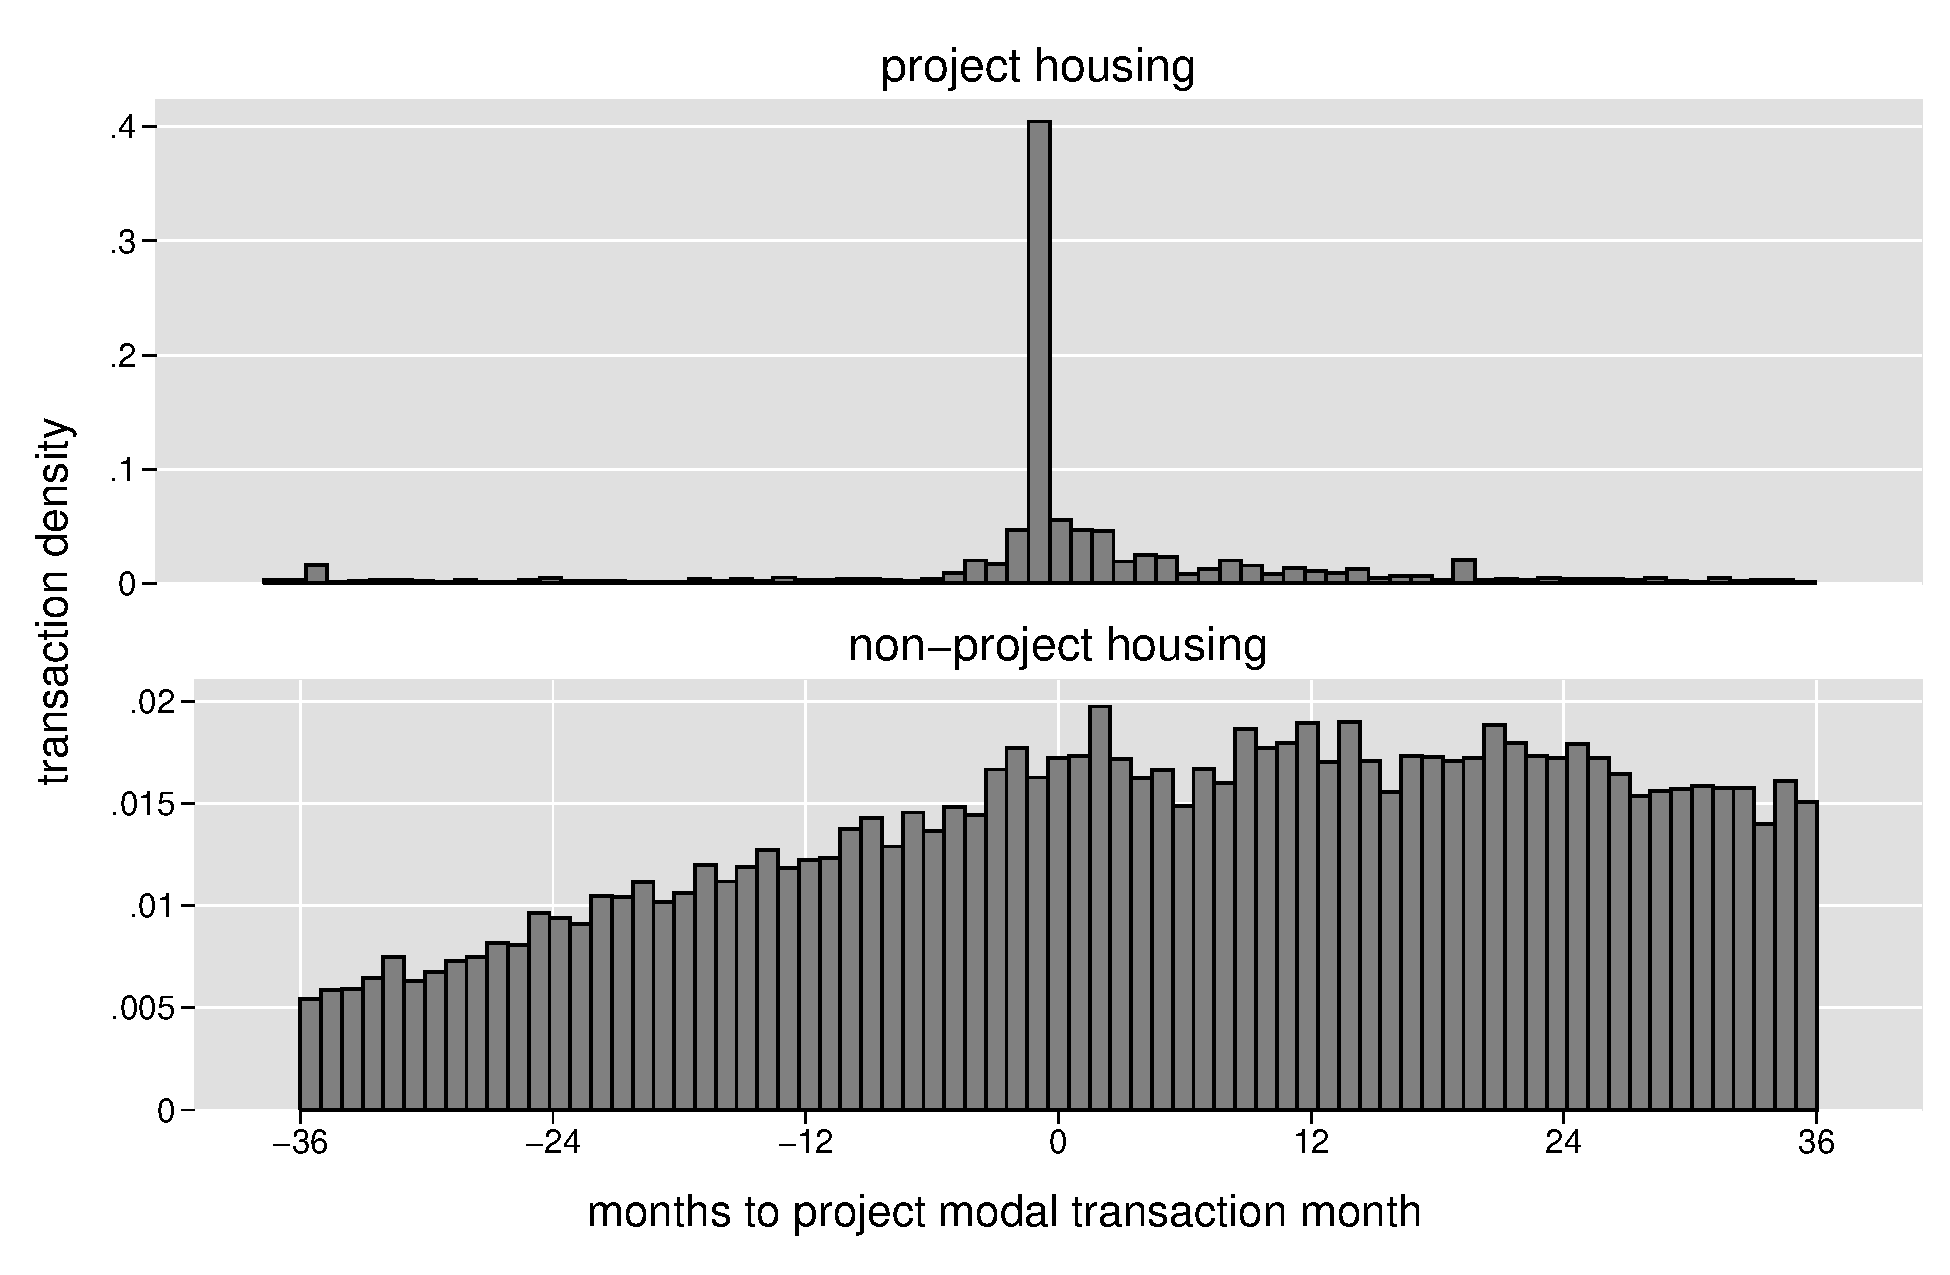
\includegraphics[scale=.4 , trim={.2cm 0.2cm .2cm 0.2cm},clip]{figures/summary_densitytime.pdf}
% \end{figure}





% \subsection{String Matching for Project Names and Delivery Dates }
% \label{appendix:stringmatch}


% We then use a fuzzy-string matching algorithm with bigrams to link project names from the budget reports to the administrative maps.  We keep all matches with over 60\% similarity, with 37 projects matching exactly.  Appendix~\ref{table:stringmatch} compares unmatched and matched projects finding that matched projects have much higher numbers of project houses, lower nearby housing prices, and are further from the central business district compared to unmatched projects.  One reason may be that the budget reports only include larger, more expansive projects, which are likely to take place further from city centers. 


% \vspace{0mm}
% \begin{table}[h!]
% \centering
% \caption{Assessing Name Matching between Budget Reports and Administrative Project Records}\label{table:stringmatch}
% \vspace{0mm}
% \begin{tabular}{l*{1}{cccc}}
% \toprule
%   & \multicolumn{2}{c}{\textbf{Matched}}& \multicolumn{2}{c}{\textbf{Unmatched}}    \\
%   &Const. & Unconst. &Const. & Unconst.  \\
% \midrule
%  Number of Projects  & 126  & 73  & 46  & 72  \\ 
 Area (km2)  & 1.22  & 1.02  & 1.05  & 1.30  \\ 
 Delivered Houses  & 416  & 15  & 259  & 7  \\ 
 House Price in 1 km (R$^\dagger$)  & 183,930  & 206,496  & 199,923  & 232,166  \\ 
 Distance to CBD$^\ddagger$ (km)  & 34.3  & 31.3  & 27.5  & 24.0  \\ 

% \bottomrule
% \multicolumn{5}{l}{\scriptsize Const. refers to constructed projects and unconst. refers to unconstructed projects.}\\[-.5em]
% \multicolumn{5}{l}{\scriptsize $^*$Calculated from {\it expected} completion dates using Gauteng National Treasury budget reports.}\\[-.5em]
% \multicolumn{5}{l}{\scriptsize $^\dagger$ The USD averaged to about 7.70 Rands during the 2001-2011 period.}\\[-.5em]
% \multicolumn{5}{l}{\scriptsize $^\ddagger$Measured as the average minimum distance with respect to Johannesburg and Pretoria CBDs. } \\[-.5em]
% \end{tabular}
% \end{table} 











% \subsection{Project counts}
% \label{appendix:projectcounts}
% \vspace{-5mm}
% \begin{figure}[ht!]
% \centering
% 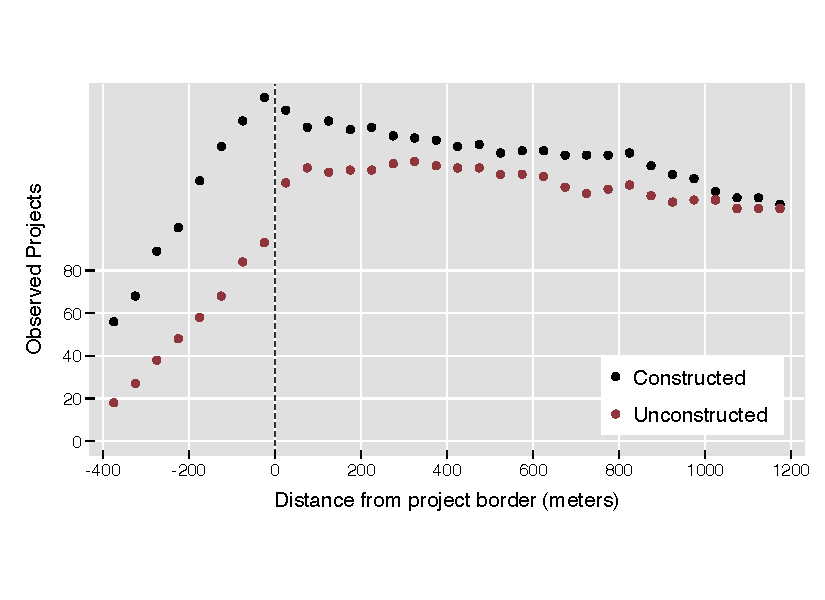
\includegraphics[scale=1.2,trim={.1cm 1.2cm .1cm 1.2cm},clip]{figures/projectcounts_4.pdf}
% \end{figure}




\end{document}


